% Nguyen Quoc Duong
\documentclass[notheorems,envcountsect,hyperref=unicode]{beamer}
\usetheme{Darmstadt}
\usefonttheme[onlylarge]{serif}
\setbeamerfont*{frametitle}{size=\normalsize,series=\bfseries}
% Standard packages
\usepackage{amsmath,amssymb,amsxtra,latexsym, amscd,amsfonts,amsthm}
\usepackage{longtable}
\usepackage[utf8]{vietnam}
\usepackage[english]{babel}
\usepackage{verbatim}
\usepackage{indentfirst}
\usepackage{multicol}
\usepackage{ragged2e}
\usepackage{color, colortbl} 
\usepackage{mathrsfs}
\usepackage{commath}
\usepackage{listings}
\usepackage{longtable} 
\usepackage{cases}
\justifying
% Setup TikZ
\usepackage{tikz}
\usetikzlibrary{arrows}
\tikzstyle{block}=[draw opacity=0.7,line width=1.4cm]
\newtheorem{nx}{Nhận xét}[section]
\newtheorem{dl}{Định lý}[section]
\newtheorem{bd}{Bổ đề} [section]
\newtheorem{dn}{Định nghĩa}[section]
\newtheorem{vd}{Ví dụ} [section]
\newtheorem{hq}{Hệ quả}[section]
\newtheorem{cm}{Chứng minh}
\newtheorem{bt}{Bài tập}
\newcommand{\R}{\mathbb R} 
\newcommand{\N}{\mathbb N} 
\newcommand{\E}{\mathbb E}
\newcommand{\Q}{\mathbb Q}
\newcommand{\Om}{\Omega}
\newcommand{\BOm}{\partial\Omega}
\DeclareUnicodeCharacter{2212}{-}
%=======================

\definecolor{dkgreen}{rgb}{0,0.6,0}             % Môi trường chứa code
\definecolor{gray}{rgb}{0.5,0.5,0.5}
\definecolor{mauve}{rgb}{0.58,0,0.82}
\lstset{frame=tb,
	language=R,
	aboveskip=3mm,
	belowskip=3mm,
	showstringspaces=false,
	columns=flexible,
	basicstyle={\small\ttfamily},
	numbers=none,
	numberstyle=\tiny\color{gray},
	keywordstyle=\color{blue},
	commentstyle=\color{dkgreen},
	stringstyle=\color{mauve},
	breaklines=true,
	breakatwhitespace=true,
	tabsize=3}
%=============================
\begin{document}
	\begin{frame}{\MakeUppercase{\textsc\bf\small{\centerline{Bộ Giáo Dục và Đào Tạo} \newline\centerline{Trường Đại Học Quy Nhơn}}}}
	\vspace*{0.2cm}
	
    \centerline{\MakeUppercase{\textsc{\bf\small{báo cáo đề tài nckh sinh viên}}}}
    \vspace*{0.2cm}
	
	\centerline{\large\alert{\MakeUppercase{\textsc{\bf{PHÂN TÍCH CHUỖI THỜI GIAN}}}}}
	\centerline{\large\alert{\MakeUppercase{\textsc{\bf{ BẰNG MÔ HÌNH ARIMA VỚI PHẦN MỀM R}}}}}
	
	\vspace*{0.2cm}
	\centerline{Sinh viên thực hiện}
	\centerline{\bf{Cao Thị Ái Loan, Phùng Thị Hồng Diễm}}
	\centerline{\bf{Nguyễn Quốc Dương, Lê Phương Thảo, Đinh Thị Quỳnh Như}}
	\vspace*{0.2cm}
	\centerline{Người hướng dẫn} \MakeUppercase{\centerline{\textsc\bf{ TS. LÊ THANH BÍNH}}}

\end{frame}
\begin{frame}
\renewcommand{\baselinestretch}{1.5}
	\frametitle{\MakeUppercase{\textsc\bf\large{Mở đầu}}}
Ngày nay, dự báo đóng một vai trò rất quan trọng trong việc hoạch định nhằm đưa ra các chính sách và chiến lược tối ưu nhất cho công việc. Có rất nhiều mô hình dự báo khác nhau như mô hình hồi quy đơn, mô hình hồi quy bội, \dots. Mỗi mô hình đều có ưu nhược điểm riêng và tùy thuộc vào đặc điểm của bộ dữ liệu đầu vào. Đối với dữ liệu có xu hướng tuyến tính và có tính dừng, mô hình ARIMA cho khả năng dự báo rất tốt. Nhằm nâng cao hiệu quả của dự báo, chúng tôi kết hợp lý thuyết mô hình ARIMA với phần mềm R để dự báo độc lập trên các tập dữ liệu thực tế. Từ kết quả dự báo, các nhà quản trị có thể tham khảo để đưa ra phương hướng tối ưu cho công việc của mình.
    \end{frame}
\begin{frame}
Nội dung báo cáo được trình bày thành 2 chương:
	\begin{itemize}
		
		\item\textbf{Chương 1. Tổng quan về lý thuyết chuỗi thời gian và mô hình ARIMA.}
		
		\item\textbf{Chương 2. Phân tích chuỗi thời gian bằng mô hình ARIMA với phầm mềm R.}
		
	\end{itemize}
\end{frame}
\begin{frame}
\frametitle{\MakeUppercase{\textsc\bf Chương 1. Tổng quan về lý thuyết chuỗi thời gian và mô hình ARIMA}}
\renewcommand{\baselinestretch}{1.5}
\begin{itemize}
  \item[1.1] \textbf{Tổng quan lý thuyết chuỗi thời gian}
\begin{itemize} 
  \item[1.1.1]\textbf{Các kiến thức mở đầu}
  \item[1.1.2]\textbf{Chuỗi thời gian có tính dừng}
  \item[1.1.3]\textbf{Hồi quy cổ điển trong chuỗi thời gian}
\end{itemize}
\item[1.2] \textbf{Mô hình ARIMA}
\begin{itemize} 
  \item[1.2.1]\textbf{Mô hình ARMA}
  \item[1.2.2]\textbf{Phương trình sai phân}
  \item[1.2.3]\textbf{Hàm ACF và PACF}
  \item[1.2.4]\textbf{Phương trình dự báo}
  \item[1.2.5]\textbf{Mô hình ARIMA}  
  \item[1.2.6]\textbf{Mô hình ARIMA theo mùa} 
\end{itemize}  
\end{itemize}
\end{frame}

\begin{frame}{1.1.1 Các kiến thức mở đầu}
\begin{block}{\textnormal{Khái niệm: Chuỗi thời gian}}
Mô tả đầy đủ của một chuỗi thời gian được quan sát như một tập hợp của $n$ biến ngẫu nhiên tại các thời điểm tùy ý $t_{1}, t_{2}, \dots, t_{n}$ (với n là số nguyên dương bất kỳ), được cho bởi hàm phân phối đồng thời, là xác suất mà mọi biến ngẫu nhiên trong chuỗi đều nhận giá trị nhỏ hơn các hằng số $c_{1}, c_{2}, \dots, c_{n},$ tức là
\begin{equation}
F(c_{1}, c_{2}, \dots, c_{n})= P(x_{t_{1}}\leq c_{1}, x_{t_{2}}\leq c_{2}, \dots, x_{t_{n}}\leq c_{n}). \label{ct1.1}
\end{equation}
\end{block}
\end{frame}

\begin{frame}{1.1.2 Chuỗi thời gian có tính dừng}
\textbf{Chuỗi có tính dừng} là một khái niệm rất quan trọng trong phân tích chuỗi thời gian. Nó được chia làm 2 loại:
\begin{itemize}
	\item Chuỗi có tính dừng ngặt
	\item Chuỗi có tính dừng yếu
\end{itemize}
 Trong bài báo cáo này, chúng tôi khai thasc đặc điểm của chuỗi có tính dừng yếu.
\end{frame}

\begin{frame}{1.1.2 Chuỗi thời gian có tính dừng}
\begin{block}{Định nghĩa: Chuỗi có tính dừng yếu \cite{1}}
\textbf{Chuỗi thời gian $x_t$ có tính dừng yếu} \textit{(tính dừng) là một quá trình phương sai hữu hạn sao cho}
\begin{itemize}
	\item[(i)]\textit{hàm giá trị trung bình $\mu_{t}$ là hằng số và không phụ thuộc vào thời gian $t$,}
	\item[(ii)]\textit{hàm hiệp phương sai $ \gamma(s, t)$ chỉ phụ thuộc vào độ sai khác $ \abs{s-t}.$} \label{dntd}
\end{itemize}
\end{block}
 Chuỗi thời gian được gọi là \textit{không có tính dừng} nếu nó không thỏa mãn được một trong các điều kiện trên.
\end{frame}

\begin{frame}{1.1.2 Chuỗi thời gian có tính dừng}
	\begin{block}{Tính chất: Phân phối mẫu lớn của ACF \cite{1}}
	\textit{Nếu $ x_{t}$ là nhiễu trắng thì ACF mẫu $\widehat{\rho_{x}}(h)$ sẽ có phân phối xấp xỉ phân phối chuẩn với giá trị trung bình bằng $0$  khi $n$ đủ lớn và độ lệch chuẩn được cho bởi
	\begin{equation}
	\sigma_{\hat{\rho}_{x}(h)}=\dfrac{1}{\sqrt{n}}, \label{ct1.40}
	\end{equation}
	trong đó $h = 1, 2, \dots, H$ với $H$ cố định nhưng tùy ý.}
	\end{block}
\end{frame}

\begin{frame}{1.1.2 Chuỗi thời gian có tính dừng}
Dựa vào kết quả trên, chúng ta có được một phương pháp để đánh giá sơ lược về ý nghĩa của các đỉnh trong $\widehat{\rho}(h)$ bằng cách xác định xem vị trí của các đỉnh được quan sát với khoảng $\pm\dfrac{2}{\sqrt{n}}$ (hoặc cộng / trừ hai lần sai số tiêu chuẩn); với một quá trình nhiễu trắng có khoảng $95\%$ các đỉnh của ACF mẫu nằm trong giới hạn này.
\end{frame}

\begin{frame}{1.1.2 Chuỗi thời gian có tính dừng}
\begin{block}{Cách xác định tính dừng của một chuỗi thời gian:}
\begin{itemize}
	\item Bằng cách \textbf{quan sát đồ thị của chuỗi thời gian}, chúng ta có thể khẳng định chuỗi $x_t$ có tính dừng nếu đồ thị của nó có \textit{xu hướng tăng hoặc giảm trong thời gian dài}.
	\item \textbf{Quan sát đồ thị ACF của chuỗi}: nếu chuỗi có tính dừng thì ACF giảm nhanh, ngẫu nhiên và không theo xu hướng; nếu chuỗi không có tính dừng thì đồ thị giảm chậm tương đối đều đặn theo độ trễ.
	\item Đối với dữ liệu không có tính dừng, \textbf{giá trị của $\hat{\rho}(h)$ (tự tương quan mẫu) tại lag 1 lớn và dương}.
	\item \textbf{Kiểm định ADF (Augmented Dickey–Fuller)}: nếu giá trị của $p$ nhỏ hơn 0.05 thì chuỗi có tính dừng và ngược lại.
\end{itemize}
\end{block}
\end{frame}

\begin{frame}{1.1.2 Chuỗi thời gian có tính dừng}
\begin{figure}[!h]
	\centering
	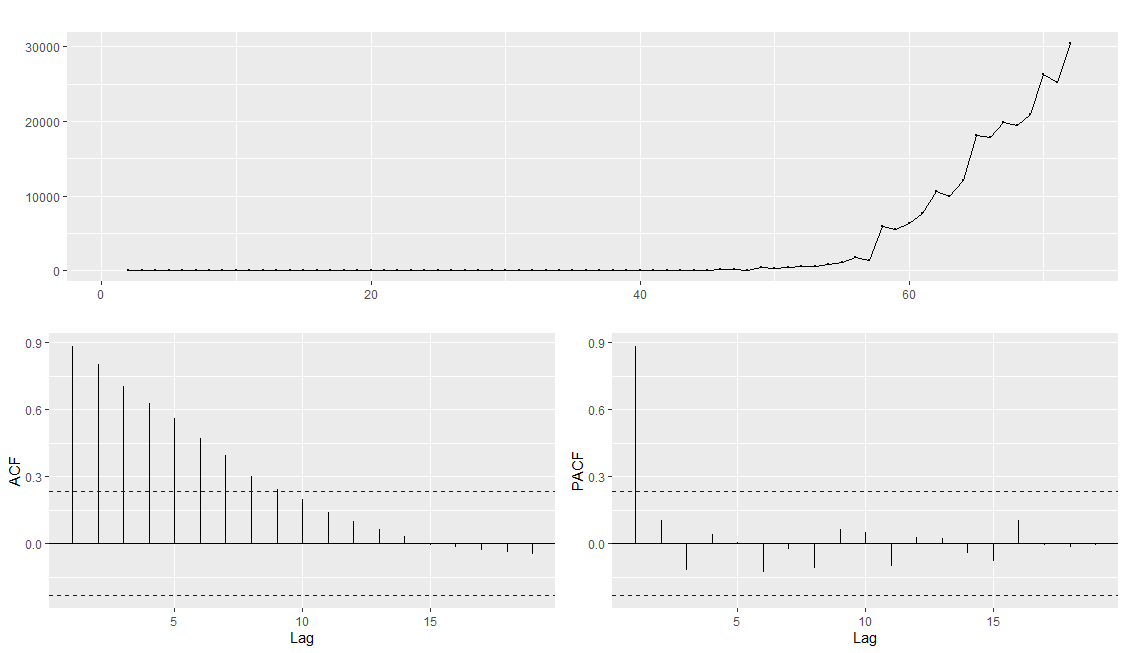
\includegraphics[width=1\linewidth,height=6cm]{U1}  
	\vskip-4mm
	\caption{Chuỗi dữ liệu số ca nhiễm mới COVID-19 theo ngày ở Mỹ}
	\label{h1}
\end{figure}
\end{frame}

\begin{frame}{1.1.2 Chuỗi thời gian có tính dừng}
	\begin{figure}[!h]
		\centering
		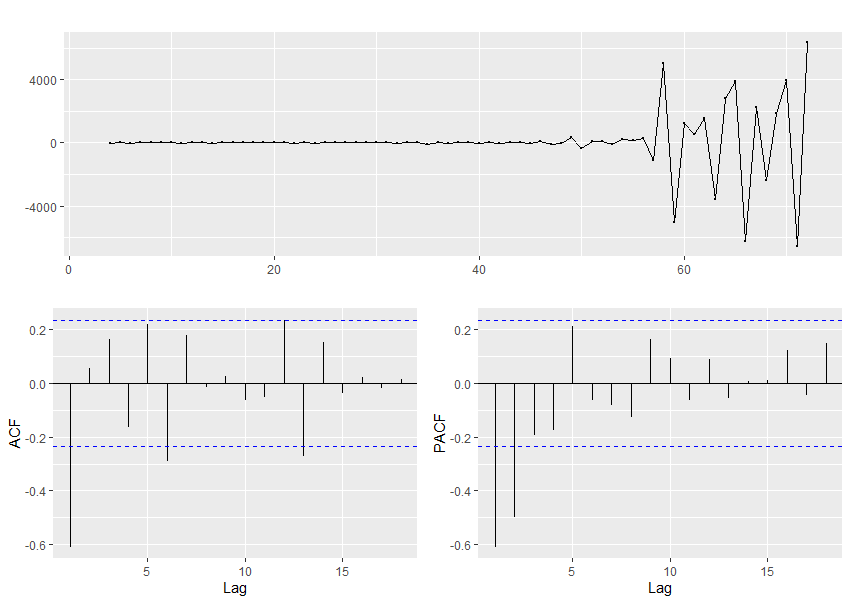
\includegraphics[width=1\linewidth,height=6cm]{U21}  
		\vskip-4mm
		\caption{Chuỗi dữ liệu số ca nhiễm mới COVID-19 theo ngày ở Mỹ}
		\label{h2}
	\end{figure}
\end{frame}

\begin{frame}{1.1.2 Chuỗi thời gian có tính dừng}
\begin{itemize}
\item Trong thực tế, phần lớn các chuỗi thời gian là chuỗi không có tính dừng. Đối với mô hình dự báo, chúng tôi cần một chuỗi ổn định. Do vậy, nếu một chuỗi thời gian không có tính dừng thì buộc chúng ta phải biến đổi chuỗi đó thành chuỗi dừng, từ đó mới có thể xây dựng được mô hình và tiến hành dự báo.
\pause
\item Có nhiều cách biến đổi chuỗi không dừng thành chuỗi dừng như dùng phép biến đổi $log$, lấy sai phân, \dots. Trong bài báo cáo này, chúng tôi sẽ đề cập đến \textit{phương pháp lấy sai phân giúp loại bỏ hoặc giảm tính không dừng của chuỗi thời gian}.
\end{itemize}
\end{frame}

\begin{frame}{1.1.2 Chuỗi thời gian có tính dừng}
	\begin{block}{Định nghĩa: \cite{1}}
Sai phân bậc 1 được ký hiệu là
\begin{equation}
\nabla x_{t}=x_{t}-x_{t-1}. \label{ct1.66}
\end{equation}
	\end{block}
\end{frame}

\begin{frame}{1.1.2 Chuỗi thời gian có tính dừng}
	\begin{block}{Định nghĩa: toán tử Backshift \cite{1}}
	\textit{\begin{align*}
			Bx_{t}=x_{t-1} 
			\end{align*}
			và mở rộng nó thành lũy thừa $$B^{2}x_{t}=B(Bx_{t})=Bx_{t-1}=Bx_{t-2}.$$ Tổng quát lên, ta được
			\begin{align*}
			B^{k}x_{t}=x_{t-k}.
			\end{align*}}
	\end{block}
\end{frame}

\begin{frame}{1.1.2 Chuỗi thời gian có tính dừng}
\begin{itemize}
	\item Phương trình sai phân bậc 1:
	\begin{align*}
	\nabla x_{t}&=x_{t}-x_{t-1}\\
	&=x_t -Bx_t=(1-B)x_{t}
	\end{align*}
	\item Phương trình sai phân bậc 2:
	\begin{align*}
	\nabla^{2} x_{t} &=(1-B)^{2}x_{t}=(1-2B+B^{2})x_{t}\\
	&=x_{t}-2x_{t-1}+x_{t-2}
	\end{align*}
	\item Phương trình sai phân bậc d:
	\begin{align*}
	\nabla^{d}=(1-B)^{d}
	\end{align*}
\end{itemize}
\end{frame}

\begin{frame}{1.1.2 Chuỗi thời gian có tính dừng}
\begin{block}{Sai phân theo mùa}
Sai phân theo mùa là sai phân giữa quan sát và quan sát tương ứng theo chu kì năm.	
\begin{align*}
\nabla x_{t}&=x_{t}-x_{t-m}
\end{align*}
trong đó $m =$ số các mùa vụ. Ví dụ, dữ liệu theo tháng thì $m = 12$, dữ liệu theo quý thì $m =4$.
\end{block}
\end{frame}

\begin{frame}{1.1.2 Chuỗi thời gian có tính dừng}
	\begin{block}{{Phân biệt các quá trình sai phân}}
		\begin{enumerate}
			\item Sai phân bậc một làm thay đổi giữa một quan sát và các quan sát tiếp theo;
			\item Sai phân theo mùa làm thay đổi một năm đến một năm tiếp theo.
		\end{enumerate}
	\end{block}
\end{frame}

\begin{frame}{1.1.2 Chuỗi thời gian có tính dừng}
\begin{block}{Chú ý \cite{3}}
Đối với chuỗi thời gian không có tính dừng và cần phải lấy sai phân và sai phân theo mùa thì
\begin{itemize}
	\item Thứ tự lấy sai phân là không quan trọng (lấy sai phân trước hay lấy sai phân theo mùa trước thì đều thu được kết quả như nhau).
	\item Nếu chuỗi dữ liệu có tính mùa vụ mạnh, chúng tôi sẽ ưu tiên lấy sai phân theo mùa trước bởi vì đôi khi kết quả của chuỗi sẽ có tính dừng ngay mà không cần phải lấy tiếp sai phân bậc 1 nữa.
\end{itemize}
\end{block}
\end{frame}

\begin{frame}{1.1.3 Hồi quy cổ điển trong chuỗi thời gian}
	\textbf{Các tiêu chuẩn thông tin \cite{1}}
	\begin{equation}
	AIC= ln (\widehat{\sigma}_{k}^{2}) +\dfrac{n+ 2k}{n} \label{ct1.60}
	\end{equation}
	\begin{equation}
	AICc= ln (\widehat{\sigma}_{k}^{2}) +\dfrac{n+ k}{n-k-2} \label{ct1.61}
	\end{equation} 
	\begin{equation}
	SIC= ln (\widehat{\sigma}_{k}^{2}) +\dfrac{kln(n)}{n} \label{ct1.62}
	\end{equation}
\end{frame}

\begin{frame}{1.1.3 Hồi quy cổ điển trong chuỗi thời gian}
	\begin{itemize}
		\item Căn của sai số bình phương trung bình (RMSE - Root Mean Squared Error):
		$$RMSE=\sqrt{MSE}=\sqrt{\frac{1}{n}\sum_{t=1}^{n}(Y_t-\hat{Y_t})^2}.$$	
		\item Sai số  tuyệt đối trung bình  (MAE - Mean Absolute Error): 
		$$ MAE=\dfrac{\mid Y_t-\hat{Y_t}\mid}{n}.$$	
		\item Sai số phần trăm tuyệt đối trung bình (MAPE - Mean Absolute Percentage Error): 
		$$MAPE=\frac{1}{n}\sum_{t=1}^{n}\mid\dfrac{ Y_t-\hat{Y_t}}{Y_t}\mid.$$
	\end{itemize}
\end{frame}

\begin{frame}{1.2 Mô hình ARIMA}
	\begin{figure}[!h]
		\centering
		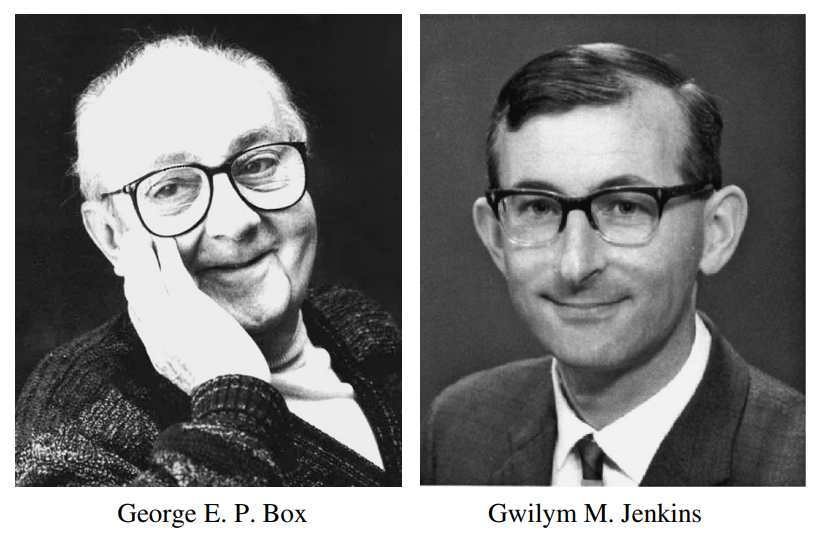
\includegraphics[width=1\linewidth,height=6cm]{box1}  
		\vskip-4mm
	\end{figure}
\end{frame}

\begin{frame}{1.2.1 Mô hình ARMA}
	\begin{block}{Định nghĩa \cite{1}}
	\textbf{Mô hình tự hồi quy bậc p}\textit{, ký hiệu là AR($p$), có dạng:
	\begin{equation}
	x_{t} = \phi_{1}x_{t-1} + \phi_{2}x_{t-2} + \dots+ \phi_{p}x_{t-p}+ w_{t}, \label{ct1.80}
	\end{equation}	
	trong đó $x_{t}$ là có tính dừng, $\phi_{1}, \phi_{2}, \dots, \phi_{p}$ là các hằng số $(\phi_{p} \neq 0)$. Trừ khi có phát biểu khác, chúng ta giả sử rằng $w_{t}$ là một chuỗi nhiễu trắng Gaussian có giá trị trung bình bằng 0 và phương sai $\sigma^{2}_w$. Khi đó giá trị trung bình của $x_t$ trong (\ref{ct1.80}) bằng 0.}
	\end{block}
\end{frame}

\begin{frame}{1.2.1 Mô hình ARMA}
\begin{block}{Định nghĩa \cite{1}}
\textit{Nếu giá trị trung bình $\mu$ của $x_{t}$ khác $0$ thì thế $x_{t}$ = $x_{t} − \mu$ vào (\ref{ct1.80}), ta được,
\begin{equation}
x_{t} − \mu= \phi_{1}(x_{t-1} - \mu) + \phi_{2}(x_{t-2}-\mu) +\dots+\phi_{p}(x_{t-p}- \mu) +w_{t}, \label{ct1.81}
\end{equation}
hoặc
\begin{equation}
x_{t}= \alpha + \phi_{1}x_{t-1} + \phi_{2}x_{t-2}+\dots+ \phi_{p}x_{t-p}+ w_{t}, \label{ct1.82}
\end{equation}
trong đó $\alpha = \mu(1-\phi_{1}-\dots-\phi_{p})$.}
\end{block}
\end{frame}


\begin{frame}{1.2.1 Mô hình ARMA}
Chúng ta cũng có thể sử dụng toán tử backshift  để viết mô hình AR($p$) (\ref{ct1.80}) dưới dạng
\begin{equation}
\phi(B)x_{t}= w_{t}, \label{ct1.84}	
\end{equation}
trong đó $\phi(B)=1-\phi_{1}B - \phi_{2}B^{2}- \dots- \phi_{p}B^{p}$ là \textit{toán tử tự hồi quy}.
\end{frame}

\begin{frame}{1.2.1 Mô hình ARMA}
	\begin{block}{Định nghĩa: \cite{1}}
\textbf{Mô hình trung bình trượt bậc q}\textit{, ký hiệu MA($q$), có dạng
	\begin{equation}
	x_{t}= w_{t}+\theta_{1}w_{t-1}+ \theta_{2}w_{t-2}+ \dots+\theta_{q}w_{t-q}, \label{ct1.100}
	\end{equation}
	với $q$ độ trễ theo trung bình trượt, $\theta_{1}, \theta_{2},\dots, \theta_{q}$  $(\theta_{q} \neq 0)$ là các tham số, $w_{t}$ là nhiễu trắng Gaussian.}
	\end{block}
\end{frame}

\begin{frame}{1.2.1 Mô hình ARMA}
Chúng ta cũng có thể viết quá trình MA($q$) ở dạng tương đương
\begin{equation}
x_{t}= \theta(B)w_{t}, \label{ct1.101}
\end{equation}
trong đó $ \theta(B)= 1+\theta_{1}B+\theta_{2}B^{2}+\dots+ \theta_{q}B^{q}$ là \textit{toán tử trung bình trượt}.
\end{frame}

\begin{frame} {1.2.1 Mô hình ARMA}
	\begin{block}{Định nghĩa: Mô hình tự hồi quy trung bình trượt ARMA(p,q)}
\textit{Một chuỗi thời gian $\{x_{t}; \hspace{0.3cm} t=0,\pm1,\pm2, \dots\}$ là} \textbf{ARMA($p$, $q$)} \textit{nếu nó có tính dừng và có dạng
	\begin{equation}
	x_{t}= \phi_{1}x_{t-1}+ \dots+\phi_{p}x_{t-p} + w_{t} + \theta_{1}w_{t-1}+ \dots+ \theta_{q}w_{t-q}, \label{ct1.104}
	\end{equation}
	với $\phi_{p} \neq 0, \theta_q \neq $0 và $\sigma_{w}^{2}> 0$; $p$ và $q$ lần lượt là bậc của tự hồi quy và trung bình trượt; $\{w_{t}; t = 0, \pm 1, \pm 2, \dots\}$ là dãy nhiễu trắng Gaussian. Nếu $x_{t}$ có giá trị trung bình $\mu \neq 0$, chúng ta đặt $\alpha = \mu(1 − \phi_{1} -\dots- \phi_{p})$ và mô hình có dạng
	\begin{equation}
	x_{t}= \alpha + \phi_{1}x_{t-1}+\dots+\phi_{p}x_{t-p}+w_{t}+\theta_{1}w_{t-1}+\dots+\theta_{q}w_{t-q}. \label{ct1.105}	
	\end{equation}}
	\end{block}
\end{frame}

\begin{frame}{1.2.1 Mô hình ARMA}
 Mô hình ARMA($p$, $q$) trong (\ref{ct1.104}) còn có thể được viết dưới dạng ngắn gọn:
\begin{equation}
\phi(B)x_{t}= \theta(B)w_{t}, \label{ct1.106}
\end{equation}
trong đó $\phi(B) $ là toán tử tự hồi quy và $\theta(B)$ là toán tử trung bình trượt.
\end{frame}

\begin{frame}{1.2.2 Phương trình sai phân}
\begin{block}{Phương trình sai phân thuần nhất bậc $p$}
Cho dãy số $u_0, u_1, u_2, \dots$, khi đó \textit{phương trình sai phân thuần nhất bậc $p$} có dạng
\begin{equation}
u_n-\alpha_1 u_{n-1}-\dots-\alpha_p u_{n-p}=0, \hspace{0.5cm}\alpha_p\neq 0, \hspace{0.5cm} n=p, p+1,\dots. \label{ct3.34}
\end{equation}
\end{block}
Đa thức liên kết là 
$$\alpha(z)=1-\alpha_1z-\dots-\alpha_pz^p.$$
\end{frame}

\begin{frame}{1.2.2 Phương trình sai phân}
	\begin{block}{Phương trình sai phân thuần nhất bậc $p$}
		Cho dãy số $u_0, u_1, u_2, \dots$, khi đó \textit{phương trình sai phân thuần nhất bậc $p$} có dạng
		\begin{equation}
		u_n-\alpha_1 u_{n-1}-\dots-\alpha_p u_{n-p}=0,  \label{ct3.34}
		\end{equation}
		với $\alpha_p\neq 0$, $n=p, p+1,\dots.$
	\end{block}
	Đa thức liên kết là 
	$$\alpha(z)=1-\alpha_1z-\dots-\alpha_pz^p.$$
\end{frame}

\begin{frame}{1.2.2 Phương trình sai phân}
Giả sử $\alpha(z)$ có $r$ nghiệm phân biệt, $z_1$ có bội $m_1$, $z_2$ có bội $m_2, \dots$, và $z_r$ có bội $m_r$, khi đó $m_1+ m_2+ \dots+ m_r=p$. Nghiệm tổng quát của phương trình sai phân (\ref{ct3.34}) là
\begin{equation}
u_n=z_1^{-n}P_1(n)+ z_2^{-n}P_{2}(n)+ \dots+ z_r^{-n}P_r(n), 
\end{equation}
trong đó $P_j(n)$ là một đa thức theo $n$ có bậc $m_j-1$, với $j = 1, 2, \dots, r$. Với $p$ điều kiện ban đầu $u_0, \dots, u_{p-1}$, chúng ta có thể tìm được $P_j(n)$.
\end{frame}


\begin{frame}{1.2.3 Hàm ACF và PACF}
ACF của một MA($q$):
\begin{align}
\rho(h) =
\begin{cases} 
\displaystyle\dfrac{\displaystyle\sum_{j=0}^{q-h}\theta_{j}\theta_{j+h}}{1+\theta_1^{2}+...+\theta_q^{2}}&, 1 \leq h \leq q\\ 
0&, h > q.\\
\end{cases}
\label{ct3.39}
\end{align}
\end{frame}

\begin{frame}{1.2.3 Hàm ACF và PACF}
Để xác định PACF cho chuỗi thời gian có tính dừng có giá trị trung bình bằng $0$, đặt $x_h^{h-1}$ là biểu diễn hồi quy của $x_{h}$ trên $\left\lbrace x_{h-1}, x_{h-2}, \dots, x_{1}\right\rbrace$, được viết dưới dạng
\begin{equation}
x_h^{h-1}= \beta_{1}x_{h-1}+ \beta_{2}x_{h-2}+ \dots+ \beta_{h-1}x_{1}. \label{ct1.128}
\end{equation}
Ngoài ra, đặt $x_0^{h-1}$ là biểu diễn hồi quy của $x_{0}$ trên $\left\lbrace x_{1}, x_{2}, \dots, x_{h-1}\right\rbrace$, khi đó 
\begin{equation}
x_0^{h-1} = \beta_{1}x_{1}+\beta_{2}x_{2}+ \dots+ \beta_{h-1}x_{h-1}. \label{ct1.129}
\end{equation}
\end{frame}

\begin{frame}{1.2.3 Hàm ACF và PACF}
	\begin{block}{Định nghĩa: Hàm PACF \cite{1}}
\textbf{Hàm tự tương quan từng phần} \textit{(PACF - Partial Auto-Correlation Function) của một quá trình dừng $x_{t}$, ký hiệu là $\phi_{hh}$, với $h=1, 2, \dots$ có dạng
	\begin{equation}
	\phi_{11}=corr(x_{1}, x_{0})=\rho(1) \label{ct1.130}
	\end{equation}	
	và 
	\begin{equation}
	\phi_{hh} = corr(x_{h}-x_h^{h-1}, x_{0}-x_0^{h-1}), \hspace{1cm} h \geq 2. \label{ct1.131}	
	\end{equation}}
	\end{block}
\end{frame}

\begin{frame}{1.2.4 Phương trình dự báo}
	\begin{block}{Tính chất \cite{1}}
\textbf{\label{BLP}Dự báo tuyến tính tốt nhất} \textit{(BLP - Best Linear Prediction) cho các quá trình có tính dừng.\\
Cho dữ liệu $x_{1}, \dots, x_{n}$, công cụ dự báo tuyến tính tốt nhất, $x_{n+m}^n= \alpha_{0} + \sum_{k=1}^{n}\alpha_{k} x_{k}$ của $x_{n+m}$, với $m\geq1$ được tìm thấy bằng cách giải
	\begin{equation}
	E[(x_{n+m} - x_{n+m}^n)x_{k}] = 0, \hspace{1cm} k=0, 1, \dots, n. \label{ct1.135}
	\end{equation}
	trong đó $x_{0}=1$.}\\
\pause
Giải phương trình (\ref{ct1.135}), ta được
\begin{equation}
x_{n+m}^{n}=\mu+\sum_{k=1}^{n}\alpha_k(x_k-\mu).
\end{equation}
	\end{block}
\end{frame}

\begin{frame}{1.2.4 Phương trình dự báo}
	\begin{block}{Dự báo trước 1 bước \cite{1}}
BLP của $x_{n+1}$ có dạng
\begin{equation}
x_{n+1}^n = \phi_{n1}x_{n}+ \phi_{n2}x_{n-1}+ \dots+ \phi_{nn}x_{1}, \label{ct1.138}
\end{equation}
Sử dụng tính chất dự báo tuyến tính tốt nhất cho các quá trình có tính dừng, các hệ số $\left\lbrace \phi_{n1}, \phi_{n2}, \dots, \phi_{nn}\right\rbrace$ thỏa mãn
$$E[(x_{n+1} - \sum_{j=1}^{n} \phi_{nj}x_{n+1-j})x_{n+1-k}] =0, \hspace{1cm} k=1, \dots, n,$$
	\end{block}
\end{frame}

\begin{frame}{1.2.4 Phương trình dự báo}
\begin{block}{Dự báo trước $m$ bước \cite{1}}
Cho dữ liệu $\left\lbrace x_{1}, \dots, x_{n}\right\rbrace$, dự báo trước $m$ bước là
\begin{equation}
x_{n+m}^{n}= \phi_{n1}^{(m)}x_{n} + \phi_{n2}^{(m)}x_{n-1}+ \dots+ \phi_{nn}^{(m)}x_{1}, \label{ct1.147}
\end{equation}	
trong đó $\{\phi_{n1}^{(m)}, \phi_{n2}^{(m)}, \dots, \phi_{nn}^{(m)}\}$ thỏa mãn phương trình dự báo
$$\sum_{j=1}^{n}\phi_{nj}^{(m)}E(x_{n+1-j}x_{n+1-k})= E (x_{n+m}x_{n+1-k}),\hspace{0.5cm} k= 1, \dots, n,$$
	\end{block}
\end{frame}

\begin{frame}{1.2.5 Mô hình ARIMA}
	\begin{block}{Định nghĩa: \cite{1}}
\textit{Một quá trình $ x_{t} $ được gọi là} \textbf{ARIMA($p$, $d$, $q$)} \textit{nếu 
	$$\nabla^{d} x_{t}=(1-B)^{d}x_{t}$$
	là ARMA($p$, $q$). Mô hình ARIMA($p$, $d$, $q$) có dạng tổng quát là
	\begin{equation}
	\phi(B)(1-B)^{d}x_{t}=\theta(B)w_{t}. \label{ct1.185}
	\end{equation} 
	Nếu $E(\nabla^{d} x_{t})=\mu$, chúng ta viết mô hình có dạng
	$$\phi(B)(1-B)^{d}x_{t}=\alpha+\theta(B)w_{t},$$
	trong đó $ \alpha=\mu(1-\phi_{1}-\dots-\phi_{p}).$}
	\end{block}
\end{frame}

\begin{frame}{1.2.5 Mô hình ARIMA}
	Mô hình ARIMA(1,1,1):
	$$ (1-\phi_1B)(1-B)x_t=\alpha+(1+\theta_1B)w_t $$
	$ \hspace{2.9cm}\uparrow\hspace{1.3cm}\uparrow\hspace{3cm}\uparrow $
	$$AR(1) \hspace{0.2cm} \text{Sai phân bậc 1} \hspace{0.7cm}MA(1) $$
	Ta có:
	$$ x_t=\alpha+\phi_{1}x_{t-1} -\phi_{1}x_{t-2} + \theta_{1}w_{t-1}+w_t $$
\end{frame}

\begin{frame}{1.2.5 Mô hình ARIMA}
	\begin{block}{Các bước để xây dựng mô hình ARIMA}
	\begin{enumerate}
	\item Kiểm tra tính dừng của chuỗi thời gian.
	\item  Chuyển một chuỗi không có tính dừng về chuỗi có tính dừng bằng cách lấy sai phân.
	\item Xác định bậc p và q.
	\item Kiểm định độ chính xác của mô hình.
	\item Dự báo.
\end{enumerate}		
	\end{block}
\end{frame}

\begin{frame}{1.2.5 Mô hình ARIMA}
	\begin{block}{Định nghĩa \cite{1}}
\textbf{Mô hình tự hồi quy trung bình trượt theo mùa} ARMA($P$, $Q$)$_s$ \textit{có dạng: 
	\begin{equation}
	\Phi_{P}(B^{s})x_{t}=\varTheta_{Q}(B^{s})w_{t}, \label{ct1.193}
	\end{equation}
	trong đó $ s $ là chu kỳ; $\Phi_ {P} (B^{s}) = 1- \Phi_{1}  B^{s}- \Phi_{2}  B^{2s}- \dots- \Phi_{P}  B^{Ps} \label{ct1.194} $ là toán tử tự hồi quy theo mùa bậc P; $\varTheta_{Q}(B^{s})= 1+ \varTheta_{1}B^{s} + \varTheta_{2}B^{2s}+ \dots+ \varTheta_{Q}B^{Qs} \label{ct1.195}	 $ là toán tự trung bình trượt theo mùa bậc Q.}
	\end{block}
\end{frame}

\begin{frame}{1.2.5 Mô hình ARIMA}
Tổng quát, chúng ta có thể kết hợp các toán tử theo mùa và không theo mùa thành mô hình tự hồi quy trung bình trượt theo mùa, được kí hiệu là ARMA$(p, q)\times(P, Q)_s$ và mô hình tổng quát được viết dưới dạng
\begin{equation}
\Phi_ {P} (B^{s})\phi(B)x_{t}= \varTheta_{Q}(B^{s})\theta(B)w_{t}. \label{ct1.196}
\end{equation}
\end{frame}

\begin{frame}{1.2.5 Mô hình ARIMA}
	\begin{block}{Định nghĩa \cite{1}}
\textit{Sai phân theo mùa bậc D} được định nghĩa là
\begin{equation}
\nabla_{s}^{D}x_{t}=(1-B^{s})^{D}x_{t}, \label{ct1.200}
\end{equation}
trong đó $D = 1, 2, \dots$. 
	\end{block}
\end{frame}

\begin{frame}{1.2.5 Mô hình ARIMA}
	\begin{block}{Định nghĩa \cite{1}}
\textbf{Mô hình tự hồi quy tích hợp trung bình trượt theo mùa}\textit{ của Box và Jenkins (1970) có dạng tổng quát là
	\begin{equation}
	\Phi_ {P} (B^{s})	\phi(B)\nabla_{s}^{D}\nabla^{d}x_{t}=\alpha + \varTheta_{Q}(B^{s})\theta(B)w_{t}, \label{ct1.201}
	\end{equation}	
	trong đó $w_{t}$ là chuỗi nhiễu trắng Gaussian. Mô hình tổng quát được ký hiệu là ARIMA $(p, d, q) \times (P, D, Q )_{s}$. Các toán tử tự hồi quy bậc $ p $ và trung bình trượt $ q $ thường được biểu thị bằng đa thức $\phi(B)$ và $\theta(B)$; toán tử tự hồi quy theo mùa  bậc $ P $ và toán tử trung bình trượt  theo mùa bậc $ Q $ lần lượt là $\Phi_ {P} (B^{s})$ và $\varTheta_{Q}(B^{s})$, và các thành phần sai phân không theo mùa và theo mùa là  $\nabla^{d}=(1-B)^{d}$ và $\nabla^{D}_{s}=(1-B^{s})^{D}$.} 
	\end{block}
\end{frame}

\begin{frame}
\frametitle{\MakeUppercase{\textsc\bf Chương 2. Phân tích chuỗi thời gian bằng mô hình ARIMA với phầm mềm R.}}
\renewcommand{\baselinestretch}{1.5}
\begin{itemize}
	\item[2.1] \textbf{Tổng quan về R và các gói lệnh} 
\item[2.2] \textbf{Phân tích dữ liệu COVID-19}
\begin{itemize}
	\item[2.2.1] \textbf{Xử lí số liệu thô.}
	\item[2.2.2] \textbf{Phân tích tổng quan COVID-19 trên toàn thế giới.}
	\item[2.2.3] \textbf{Dự báo số ca nhiễm mới COVID-19 tại Mỹ.}
	\item[2.2.4] \textbf{Dự báo số ca tử vong mới COVID-19 tại Italy.}  	  	
\end{itemize}
\item[2.3] \textbf{Phân tích và dự báo lượng mưa tại trạm quan trắc Quy Nhơn}
\item[2.4] \textbf{Website dashboard COVID-19 với Shinyapps}
\end{itemize}
\end{frame}

\begin{frame}{2.1 Tổng quan về R và các gói lệnh}
\textbf{Tổng quan về R}\\
\begin{itemize}
	\item Phân tích thống kê và đồ thị.
	\item Mã nguồn mở, miễn phí.
	\item Có đầy đủ tính năng của các phần mềm thương mại đắt tiền như SPSS, AMOS, STATA hay EViews và nó có tính năng vượt trội hơn hẳn.
	\item Công cụ cho Data Mining, Big Data, Data Visualization và Machine Learning.
	\item Năm 1996,  hai nhà thống kê học Ross Ihaka và Robert Gentleman thuộc Trường đại học Auckland, New Zealand phát hoạ ra ngôn ngữ R.
\end{itemize}
\end{frame}

\begin{frame}{2.1 Tổng quan về R và các gói lệnh}
\textbf{Các gói lệnh được sử dụng trong bài báo cáo}\\
\begin{itemize}
	\item Gói lệnh "forecast" của Rob Hyndman và các cộng sự (Version 8.12 - 2020).
	\item Gói lệnh "ggplot2" dùng để vẽ biểu đồ với đa dạng lựa chọn với nhiều tùy biến.
	\item Gói lệnh "magrittr" chứa các toán tử.
	\item Gói lệnh "gridExtra" dùng để chưa các ảnh dưới dạng lưới.
	\item Gói lệnh "kableExtra" dùng để chuyển dữ liệu bảng từ R sang code Latex với nhiều tùy chỉnh.
\end{itemize}
\end{frame}

\begin{frame}{2.2 Phân tích dữ liệu COVID-19}
	\begin{figure}[!h]
		\centering
		
\includegraphics[width=1\linewidth,height=6cm]{covid19}  
		\vskip-4mm
	\end{figure}
\end{frame}

\begin{frame}{2.2.1 Xử lý dữ liệu thô}
\begin{itemize}
\item Chúng tôi lấy dữ liệu toàn cầu dưới dạng thô được thống kê hàng ngày của Johns Hopkins CSSE tại \url{https://github.com/CSSEGISandData/COVID-19}.
\item Các nguồn dữ liệu được thống kê bao gồm Tổ chức Y tế Thế giới (WHO), Trung tâm Kiểm soát và Phòng ngừa Dịch bệnh Hoa Kỳ (CDC) và Ủy ban Y tế Quốc gia của Cộng hòa Nhân dân Trung Hoa (NHC).
\item Dữ liệu này được thu thập bởi Đại học Johns Hopkins, được phát triển bởi nhóm ESRI Living Atlas.
\end{itemize}
\end{frame}

\begin{frame}{2.2.2 Phân tích tổng quan COVID-19 trên toàn thế giới.}
\begin{figure}[!htb]
	\centering
	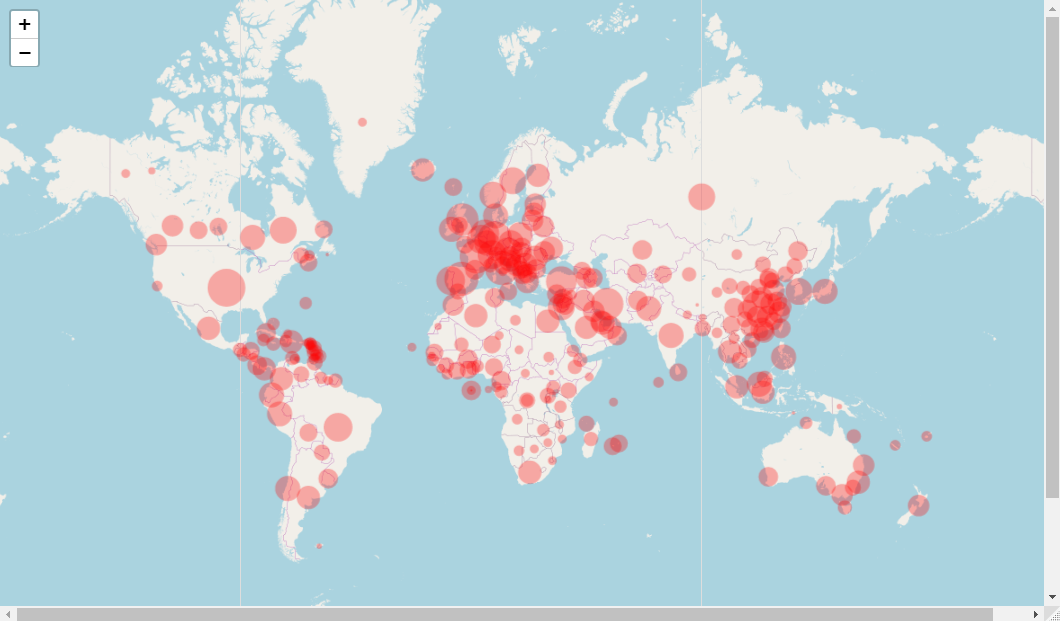
\includegraphics[width=1\linewidth,height=6cm]{Rplot}  
	\caption{Bản đồ phân bố dịch COVID-19 trên toàn thế giới (7/4/2020)}
\end{figure}
\end{frame}

\begin{frame}{2.2.2 Phân tích tổng quan COVID-19 trên toàn thế giới.}
\begin{figure}[t]
	\centering
	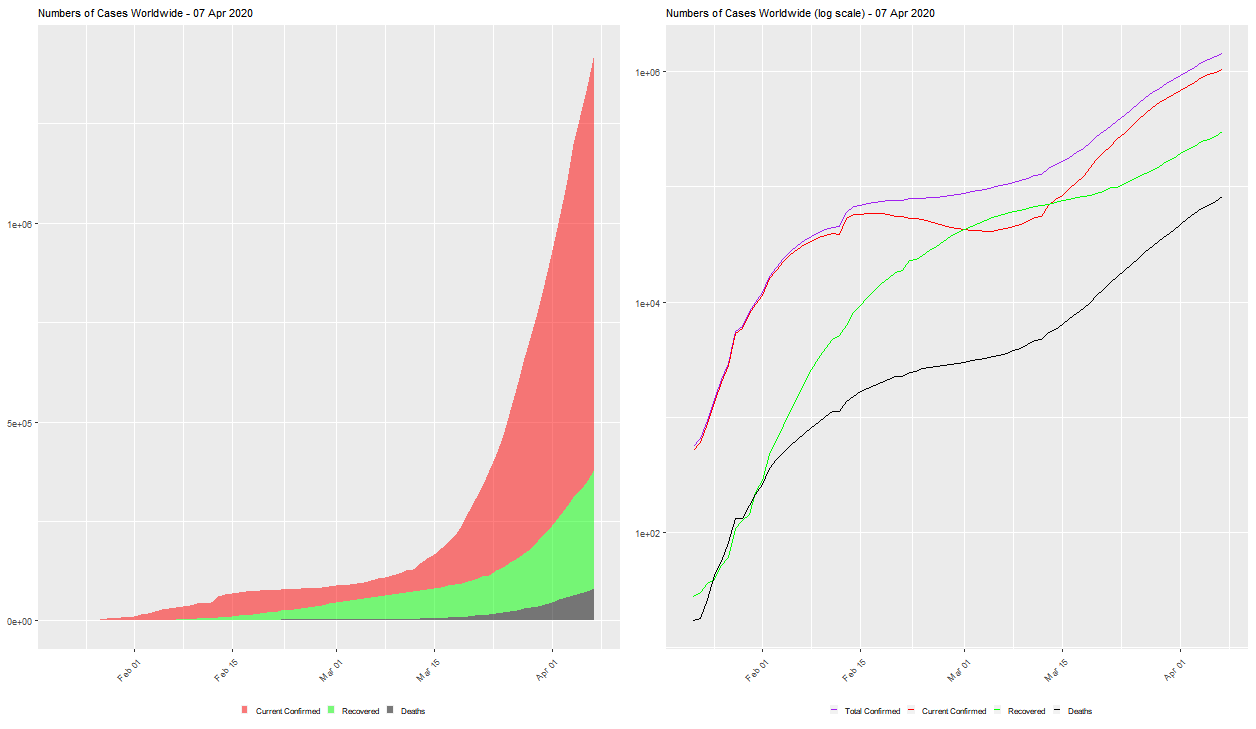
\includegraphics[width=1\linewidth,height=6cm]{Rplot01}  
	\caption{Đồ thị dữ liệu COVID-19 trên toàn thế giới (7/4/2020)}
\end{figure}
\end{frame}

\begin{frame}{2.2.2 Phân tích tổng quan COVID-19 trên toàn thế giới.}
\begin{figure}[t]
	\centering
	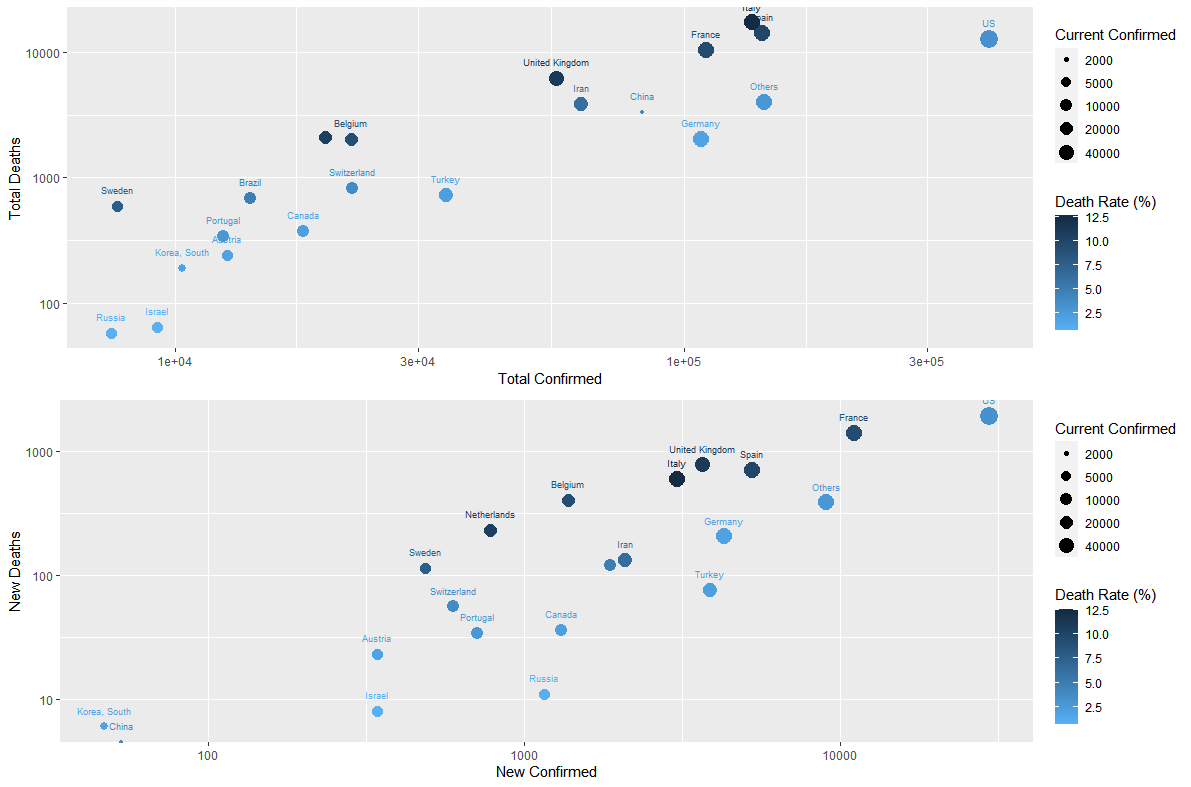
\includegraphics[width=1\linewidth,height=6.5cm]{Rplot02}  
	\caption{Top 20 quốc gia (7/4/2020)}
\end{figure}
\end{frame}

\begin{frame}{2.2.2 Phân tích tổng quan COVID-19 trên toàn thế giới.}
Các nghiên cứu sử dụng mô hình ARIMA như là một công cụ hữu ích trong việc theo dõi và dự báo xu hướng thay đổi trong các bệnh truyền nhiễm.
\pause
\begin{itemize}
\item L.LIU và các cộng sự của mình đã sử dụng mô hình ARIMA để dự báo tỷ lệ mắc bệnh tay, chân, miệng ở tỉnh Tứ Xuyên, Trung Quốc \cite{10}.
\pause
\item Li và các cộng sự đã áp dụng mô hình ARIMA để dự báo tỷ lệ mắc bệnh sốt xuất huyết tại tỉnh Lâm Nghi, Trung Quốc \cite{11}.
\pause
\item Earnest cùng các cộng sự đã dùng mô hình ARIMA như một công cụ hữu ích cho quản trị viên và các bác sỹ trong việc lập kế hoạch phân bố giường bệnh cho các bệnh nhân trong đợt dịch SARS bùng phát \cite{12}.
\end{itemize}
\end{frame}

\begin{frame}{2.2.3 Dự báo số ca nhiễm mới COVID-19 tại Mỹ.}
Tình hình nước Mỹ:
	\pause
	\begin{itemize}
		\item hơn 350000 ca nhiễm và gần 1300 ca tử vong (tính tại thời điểm ngày 7/4/2020). Hoa Kỳ trở thành tâm điểm toàn cầu của đại dịch khi vượt qua số ca nhiễm ở Trung Quốc - nơi mầm bệnh của COVID-19.
		\pause
		\item Hoa Kỳ là một trong những quốc gia có nền y tế phát triển bậc nhất thế giới tuy nhiên vẫn tồn tại một số lỗ hổng nhất định.
		\pause
		\item COVID-19 xuất hiện vào thời điểm trọng yếu của chính trị Mỹ nên động thái xử lý dịch bệnh chậm trễ và thiếu dứt khoát ngay từ đầu.
	\end{itemize}
$\Longrightarrow$ Dự báo diễn biến tình hình dịch bệnh ở Mỹ là việc hết sức quan trọng và cần thiết.
\end{frame}

\begin{frame}{2.2.3 Dự báo số ca nhiễm mới COVID-19 tại Mỹ.}
	\begin{figure}[!htb]
		\centering
		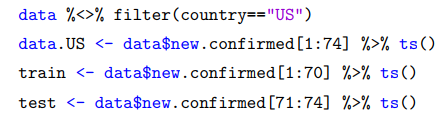
\includegraphics[width=1\linewidth,height=3.5cm]{t1} 
	\end{figure}
\end{frame}

\begin{frame}{2.2.3 Dự báo số ca nhiễm mới COVID-19 tại Mỹ.}
\textbf{Bước 1: Kiểm tra tính dừng của tập "train"}
\begin{figure}[!htb]
	\centering
	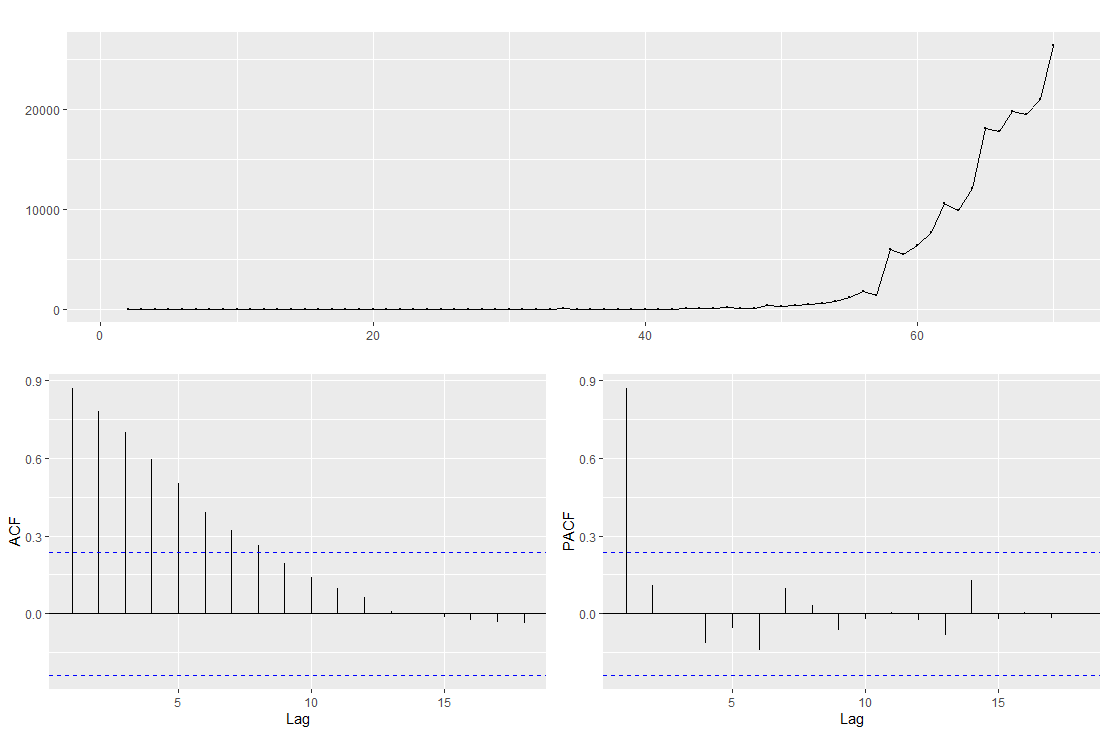
\includegraphics[width=1\linewidth,height=6cm]{US1}
	\caption{Đồ thị ACF và PACF của tập "train"}  
\end{figure}
\end{frame}

\begin{frame}{2.2.3 Dự báo số ca nhiễm mới COVID-19 tại Mỹ.}
\begin{figure}[!htb]
	\centering
	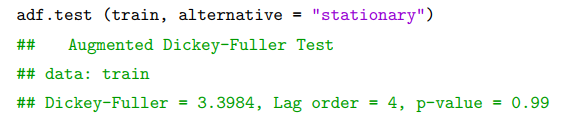
\includegraphics[width=1\linewidth,height=3.5cm]{d1} 
\end{figure}
\end{frame}

\begin{frame}{2.2.3 Dự báo số ca nhiễm mới COVID-19 tại Mỹ.}
	\textbf{Bước 2: Chuyển đổi chuỗi không có tình dừng thành chuỗi có tính dừng}
	\begin{figure}[!htb]
		\centering
		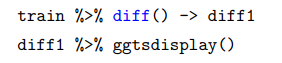
\includegraphics[width=1\linewidth,height=2cm]{t2} 
	\end{figure}
\end{frame}

\begin{frame}{2.2.3 Dự báo số ca nhiễm mới COVID-19 tại Mỹ.}
	\begin{figure}[!htb]
		\centering
		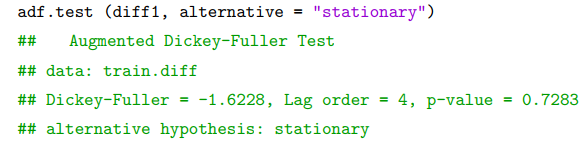
\includegraphics[width=1\linewidth,height=3.5cm]{d2} 
	\end{figure}
\end{frame}

\begin{frame}{2.2.3 Dự báo số ca nhiễm mới COVID-19 tại Mỹ.}
	\begin{figure}[!htb]
		\centering
		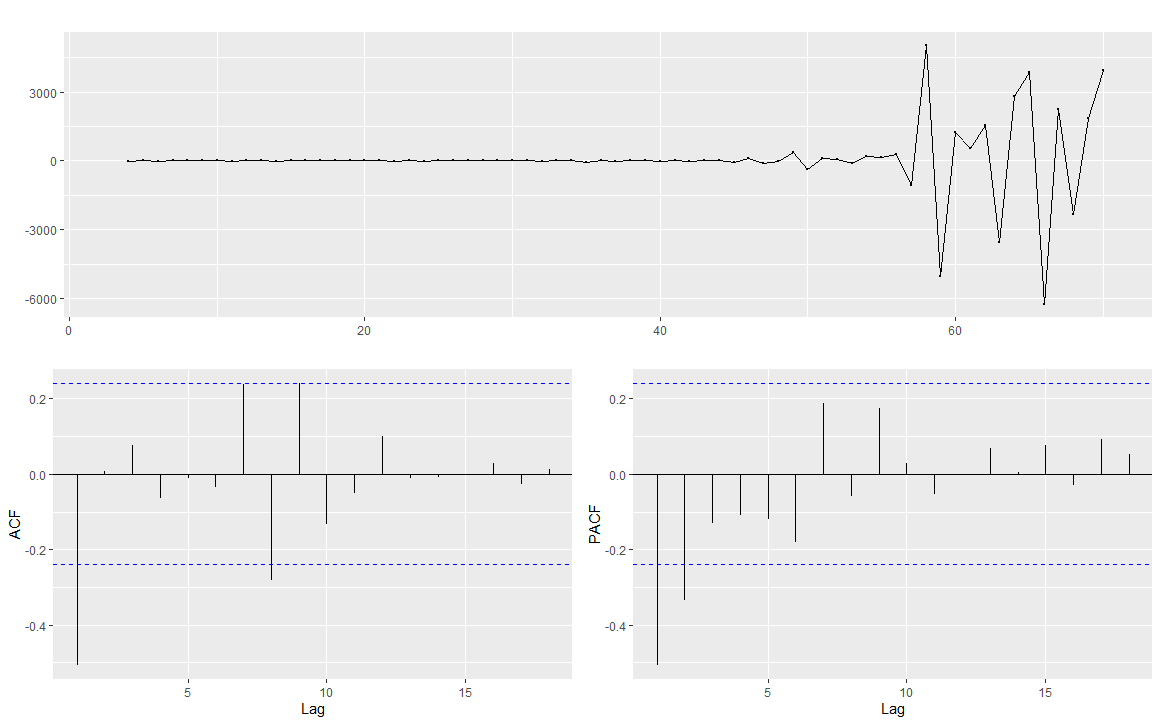
\includegraphics[width=1\linewidth,height=6cm]{US2} 
	\end{figure}
\end{frame}

\begin{frame}{2.2.3 Dự báo số ca nhiễm mới COVID-19 tại Mỹ.}
	\begin{figure}[!htb]
		\centering
		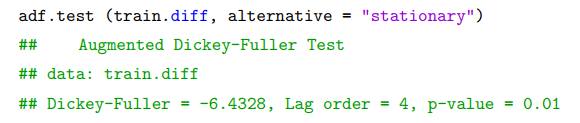
\includegraphics[width=1\linewidth,height=3.5cm]{d3} 
	\end{figure}
Kết quả của kiểm tra ADF cho thấy $p-value = 0.01 < 0.05$ $\Longrightarrow$ Chuỗi tập "train" có tính dừng sau khi lấy sai phân bậc 2.
\end{frame}

\begin{frame}{2.2.3 Dự báo số ca nhiễm mới COVID-19 tại Mỹ.}
	\begin{figure}[!htb]
		\centering
		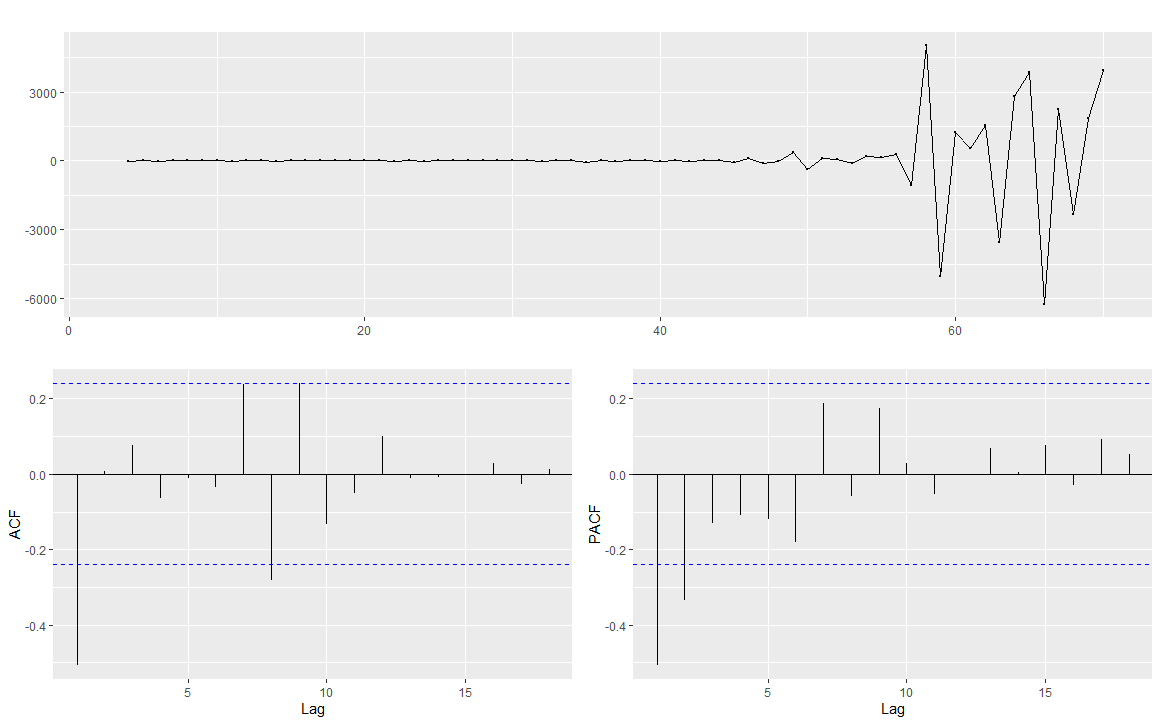
\includegraphics[width=1\linewidth,height=5.5cm]{US2} 
	\end{figure}
\pause
$\Longrightarrow$  Mô hình đơn giản từ đồ thị ACF là ARIMA(0, 2, 2)\\ $\Longrightarrow$  \pause $AICc= 1116.71$
\end{frame}

\begin{frame}{2.2.3 Dự báo số ca nhiễm mới COVID-19 tại Mỹ.}
\textbf{Bước 4: Khớp và chọn mô hình phù hợp nhất}
	\begin{figure}[!htb]
	\centering
	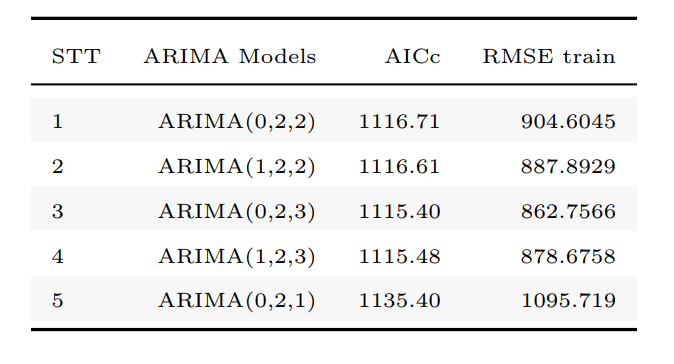
\includegraphics[width=1\linewidth,height=5.5cm]{bus1} 
\end{figure}
$\Longrightarrow$ Mô hình ARIMA(0, 2, 3) là mô hình phù hợp nhất (AICc và RMSE nhỏ nhất).
\end{frame}

\begin{frame}{2.2.3 Dự báo số ca nhiễm mới COVID-19 tại Mỹ.}
\textbf{Bước 5: Kiểm tra phần dư từ mô hình được chọn}
	\begin{figure}[!htb]
		\centering
		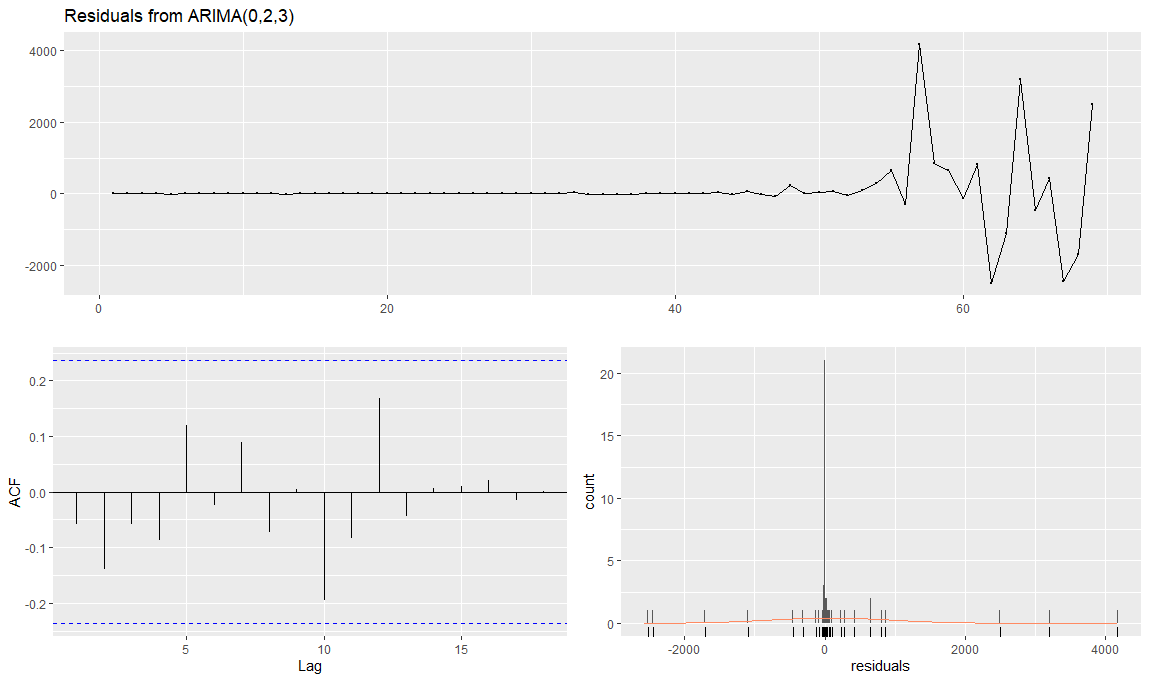
\includegraphics[width=1\linewidth,height=5.5cm]{NT1} 
	\end{figure}
\end{frame}

\begin{frame}{2.2.3 Dự báo số ca nhiễm mới COVID-19 tại Mỹ.}
	\textbf{Bước 5: Đánh giá sai số của mô hình ARIMA(0,2,3) và dự báo}
	\begin{figure}[!htb]
		\centering
		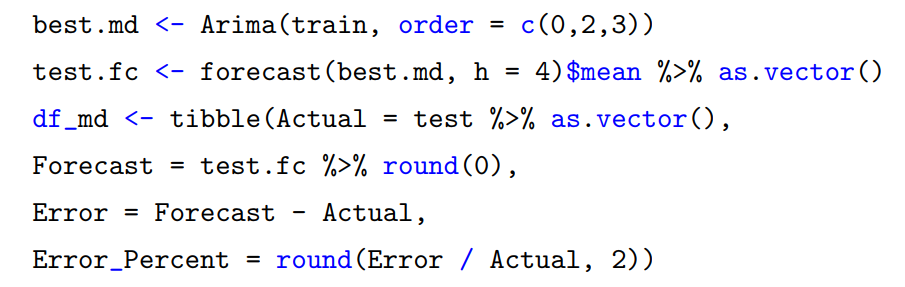
\includegraphics[width=1\linewidth,height=5.5cm]{duong1} 
	\end{figure}
\end{frame}

\begin{frame}{2.2.3 Dự báo số ca nhiễm mới COVID-19 tại Mỹ.}
	\begin{figure}[!htb]
		\centering
		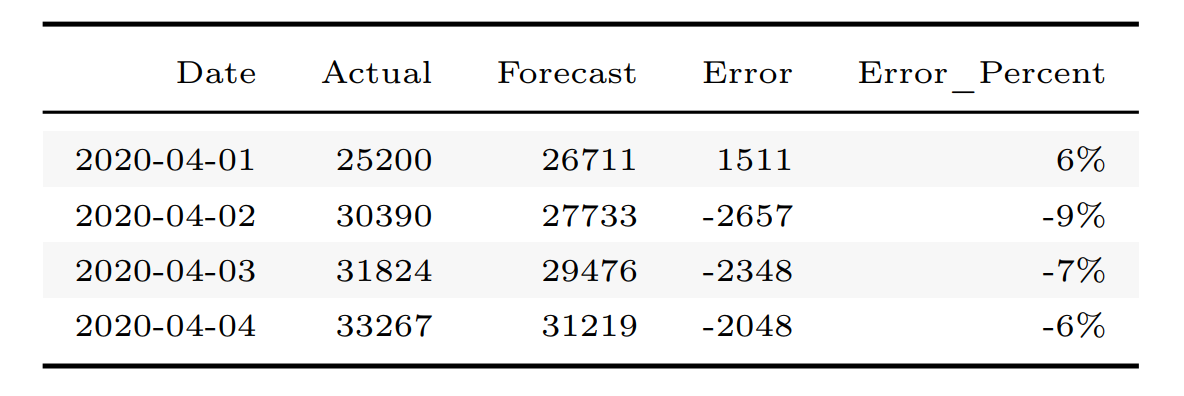
\includegraphics[width=1\linewidth,height=5.5cm]{duong2} 
	\end{figure}
\end{frame}

\begin{frame}{2.2.3 Dự báo số ca nhiễm mới COVID-19 tại Mỹ.}
	\begin{figure}[!htb]
		\centering
		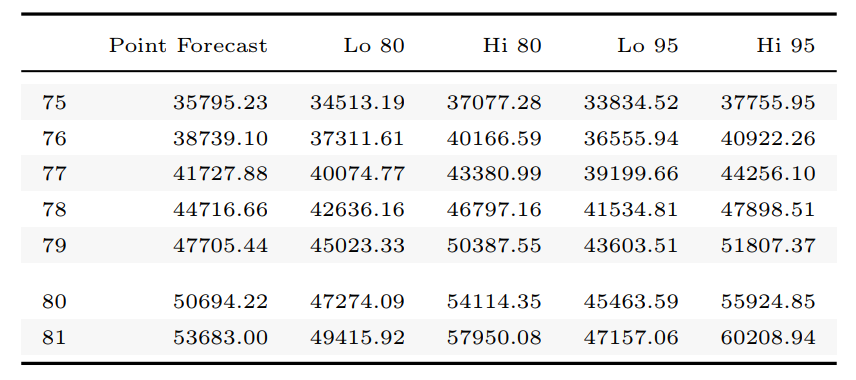
\includegraphics[width=1\linewidth,height=5.5cm]{duong3} 
	\end{figure}
\end{frame}

\begin{frame}{2.2.3 Dự báo số ca nhiễm mới COVID-19 tại Mỹ.}
	\begin{figure}[!htb]
		\centering
		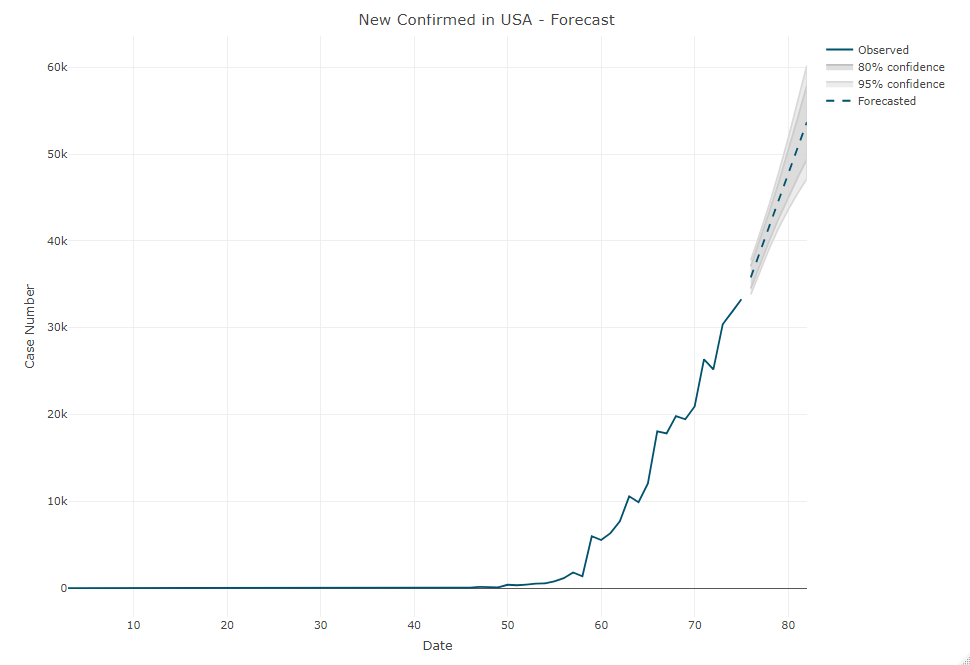
\includegraphics[width=1\linewidth,height=5.5cm]{A7} 
	\end{figure}
\end{frame}

\begin{frame}{2.2.4 Dự báo số ca tử vong mới COVID-19 tại Ý.}
\textbf{Tình hình COVID-19 tại Ý}\\
\begin{itemize}
	\item Cơ quan Bảo vệ Dân sự xác nhận thêm 3.039 ca dương tính với SARS-CoV-2 trong ngày 7/4. Mặc dù đây là số ca nhiễm mới thấp nhất kể từ ngày 17/3 tại quốc gia này, nhưng số ca tử vong lại tăng lên rất cao.
	\item Có thêm 604 ca tử vong do SARS-CoV-2 ở Italy, nâng tổng số bệnh nhân COVID-19 thiệt mạng lên đến 17.127 người - mức cao nhất trên thế giới.
\end{itemize}
\pause
\textbf{Vậy nguyên nhân dẫn đến sự tăng vọt này là gì?}
\end{frame}

\begin{frame}{2.2.4 Dự báo số ca tử vong mới COVID-19 tại Ý.}
Nhóm Ioannidis vừa có một bài báo được đăng trên tạp chí JAMA Int Med đưa ra những quan điểm trả lời cho câu hỏi trên \cite{16}.
\begin{itemize}
	\item Yếu tố lão hóa dân số: Ý có dân số già bậc nhất châu Âu. Gần một phần tư (23\%) dân số của nước này có độ tuổi từ 65 trở lên. Hơn thế, những người này tiền sử bệnh như hô hấp, tim mạch, tiểu đường và ung thư. Do đó, gánh nặng dịch bệnh đã đè lên bệnh trạng sẵn có.
	\item Hệ thống y tế: mặc dù Ý là nước có hệ thống y tế Nhà nước rất tốt, nhưng số giường bệnh ICU thì rất khiêm tốn (toàn quốc chỉ có 5090 giường, tức 8.4 trên 100,000 dân).
\end{itemize}
\end{frame}

\begin{frame}{2.2.4 Dự báo số ca tử vong mới COVID-19 tại Ý.}
	\begin{figure}[!htb]
	\centering
	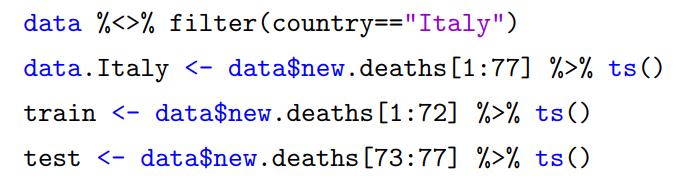
\includegraphics[width=1\linewidth,height=4cm]{duong4} 
\end{figure}
\end{frame}

\begin{frame}{2.2.4 Dự báo số ca tử vong mới COVID-19 tại Ý.}
\textbf{Bước 1: Vẽ đồ thị số ca tử vong mới tại Ý trên tập "train"}\\
	\begin{figure}[!htb]
		\centering
		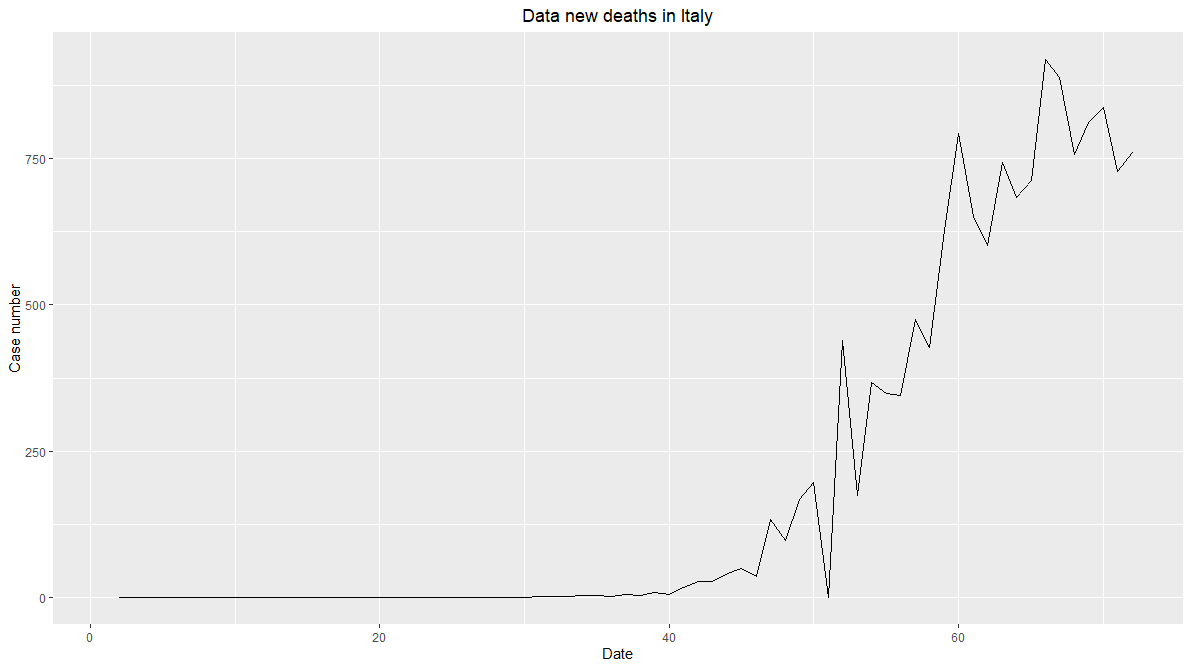
\includegraphics[width=1\linewidth,height=5cm]{I1} 
	\end{figure}
\end{frame}

\begin{frame}{2.2.4 Dự báo số ca tử vong mới COVID-19 tại Ý.}
\textbf{Bước 2: Sử dụng hàm "auto.arima" để tìm ra mô hình tốt nhất}\\
	\begin{figure}[!htb]
		\centering
		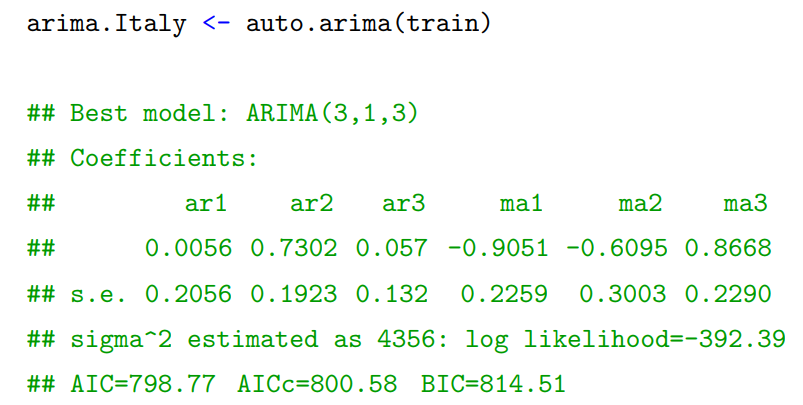
\includegraphics[width=1\linewidth,height=5cm]{duong5} 
	\end{figure}
\end{frame}

\begin{frame}{2.2.4 Dự báo số ca tử vong mới COVID-19 tại Ý.}
\textbf{Bước 3: Kiểm tra phần dư từ mô hình ARIMA(3,1,3)}\\
	\begin{figure}[!htb]
		\centering
		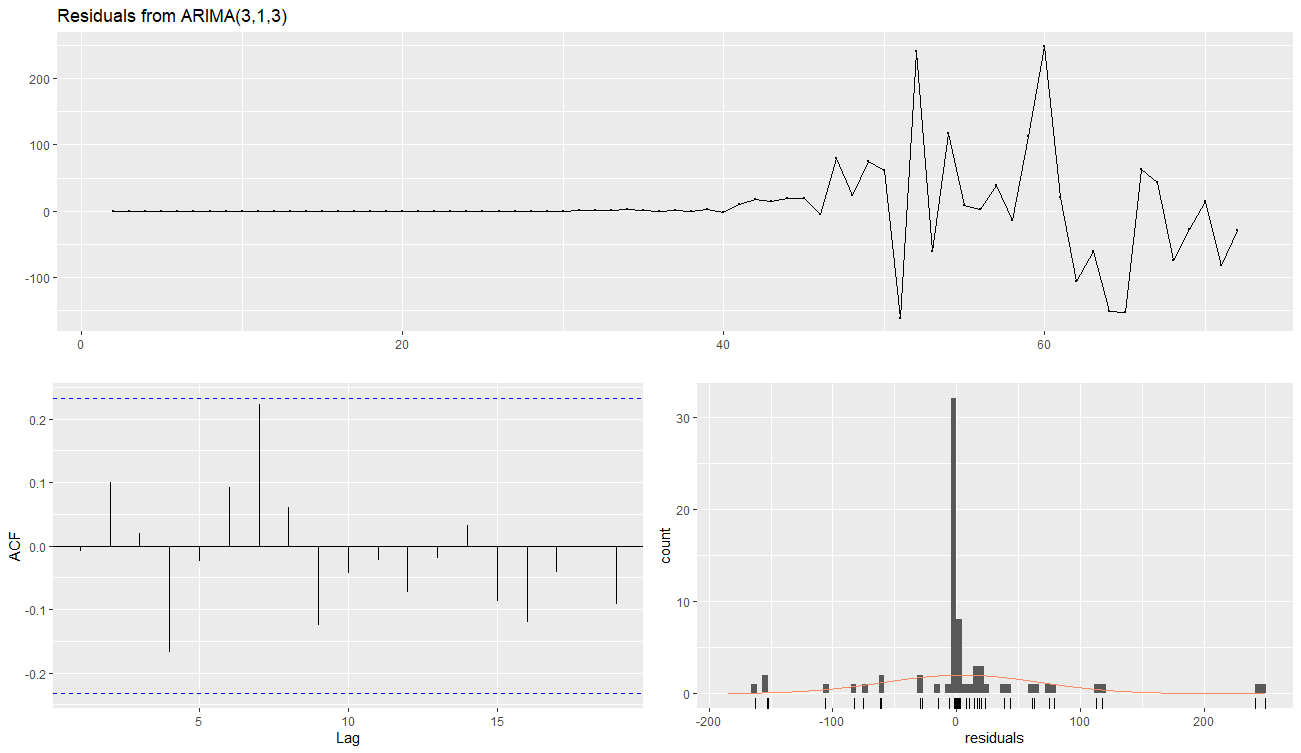
\includegraphics[width=1\linewidth,height=5cm]{PD1} 
	\end{figure}
\end{frame}

\begin{frame}{2.2.4 Dự báo số ca tử vong mới COVID-19 tại Ý.}
\textbf{Bước 4: Đánh giá sai số từ mô hình ARIMA(3,1,3) và dự báo}\\
	\begin{figure}[!htb]
		\centering
		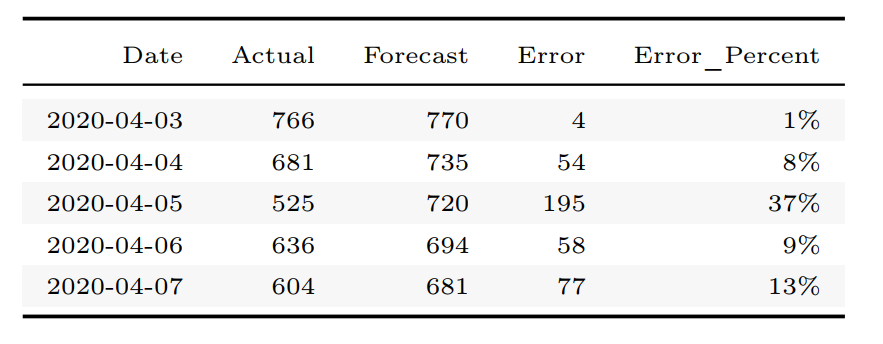
\includegraphics[width=1\linewidth,height=5cm]{duong6} 
	\end{figure}
\end{frame}

\begin{frame}{2.2.4 Dự báo số ca tử vong mới COVID-19 tại Ý.}
	\begin{figure}[!htb]
		\centering
		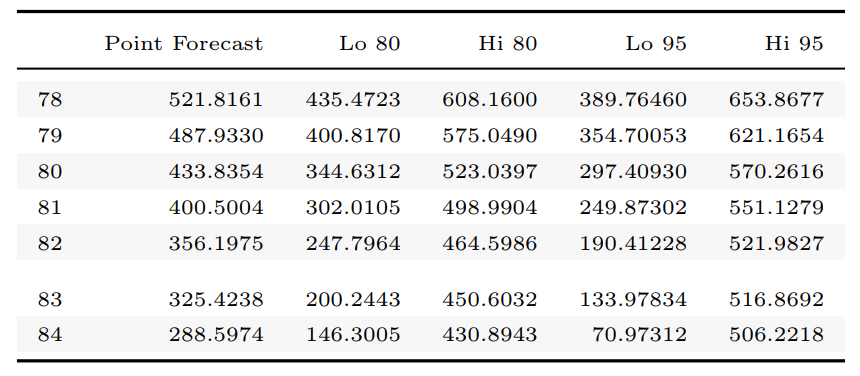
\includegraphics[width=1\linewidth,height=5.5cm]{duong7} 
	\end{figure}
\end{frame}

\begin{frame}{2.2.4 Dự báo số ca tử vong mới COVID-19 tại Ý.}
	\begin{figure}[!htb]
		\centering
		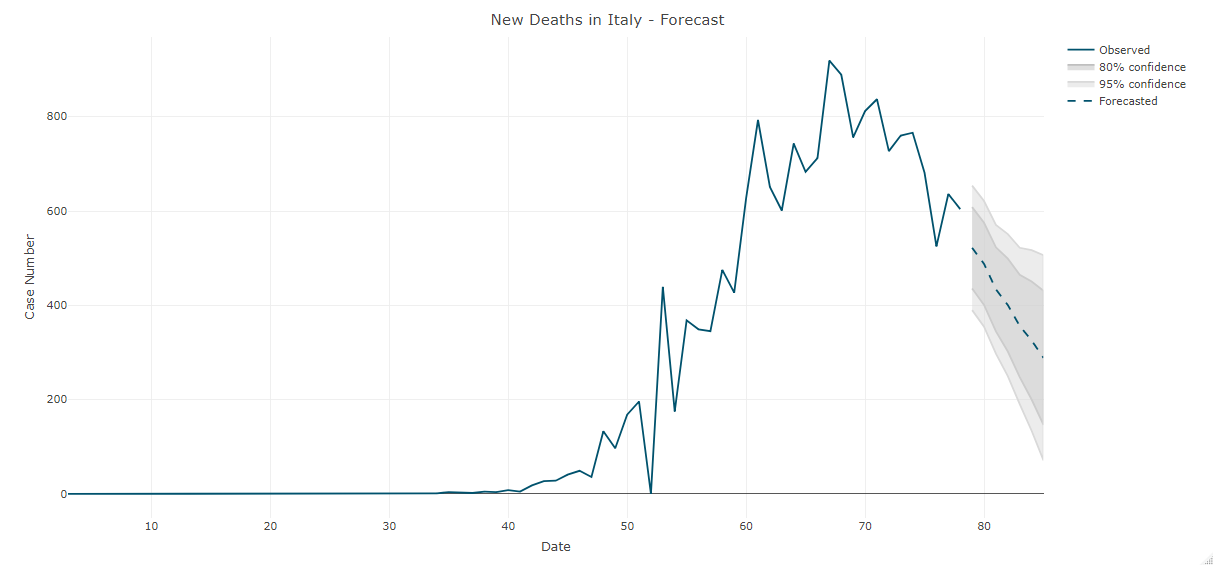
\includegraphics[width=1\linewidth,height=5.5cm]{A8} 
	\end{figure}
\end{frame}

\begin{frame}{2.3 Phân tích và dự báo lượng mưa tại trạm quan trắc Quy Nhơn.}
\textbf{Lợi ích của việc dự báo lượng mưa?}\\
\begin{itemize}
\item Lượng mưa là một trong những hiện tượng quan trọng nhất của hệ thống tự nhiên có ảnh hưởng chung đến biến đổi khí hậu.
\item Do đó, việc mô hình hóa và dự báo nó là cần thiết để giải quyết một số vấn đề liên quan đến quy hoạch và quản lí hệ thống tài nguyên nước, công trình thủy lợi, quản lí nông nghiệp, ...
\end{itemize}
\end{frame}

\begin{frame}{2.3 Phân tích và dự báo lượng mưa tại trạm quan trắc Quy Nhơn.}
	\textbf{Các nghiên cứu sử dụng ARIMA theo mùa để dự báo lượng mưa}\\
	\begin{itemize}
		\item Rahman và các cộng sự đã có một bài nghiên cứu đánh giá giữa 2 mô hình ARIMA và ANFIS để dự báo thời tiết cho thành phố Dhaka, kết quả cho thấy mô hình ARIMA thực hiện tốt hơn ANFIS \cite{18}.
		\item Dizon công bố kết quả nghiên cứu về ARIMA theo mùa là một mô hình rất tốt cho dự báo chuỗi thời gian có tính mùa vụ mạnh \cite{19}. Momani sử dụng thành công mô hình ARIMA để dự báo xu hướng lượng mưa của Jordan \cite{20}.
		\item Tại Việt Nam, Nguyễn Hữu Quyền đã có một bài luận văn thạc sĩ khoa học về ứng dụng mô hình động thái ARIMAX để dự báo lượng mưa vụ đông xuân ở một số tỉnh vùng đồng bằng Bắc Bộ.
	\end{itemize}
\end{frame}

\begin{frame}{2.3 Phân tích và dự báo lượng mưa tại trạm quan trắc Quy Nhơn.}
Chúng tôi lấy dữ liệu của trạm quan trắc Quy Nhơn từ \textit{Trung tâm dữ liệu khí tượng thủy văn quốc gia} (\url{http://cmh.com.vn/}). Dữ liệu được thống kê từ tháng 1/2000 đến tháng 12/2018.
\end{frame}

\begin{frame}{2.3 Phân tích và dự báo lượng mưa tại trạm quan trắc Quy Nhơn.}
\textbf{Đặc điểm lượng mưa tại trạm quan trắc Quy Nhơn}
\begin{figure}[!htb]
	\centering
	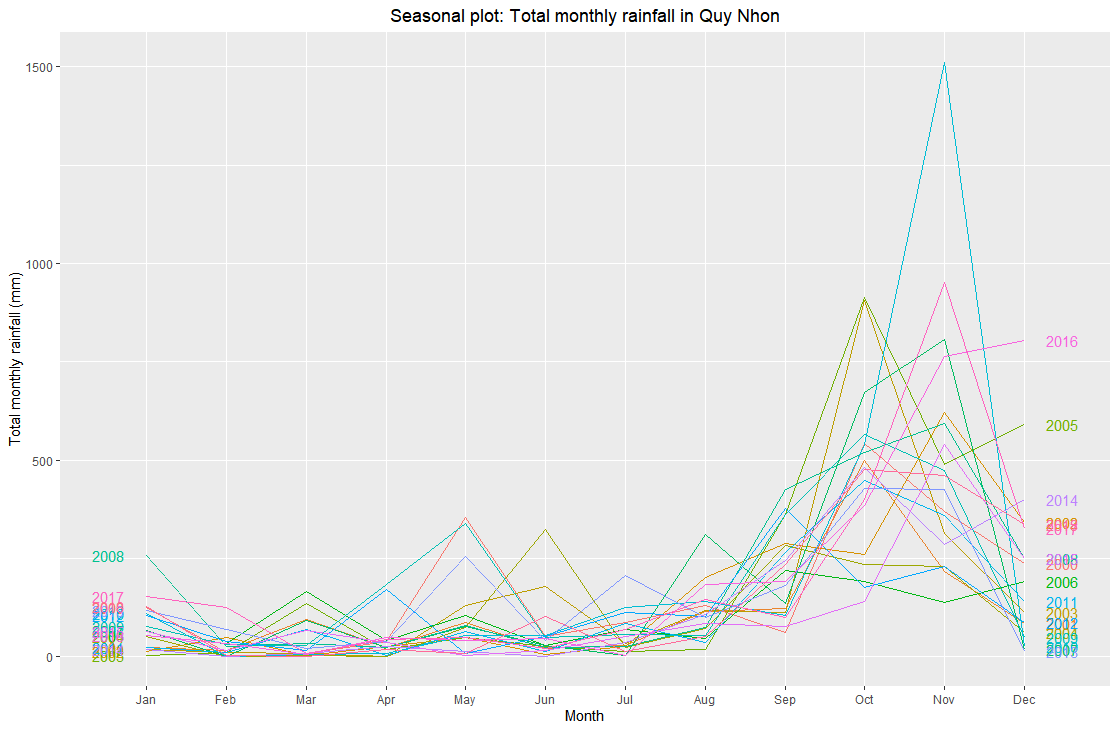
\includegraphics[width=1\linewidth,height=6cm]{V2} 
\end{figure}
\end{frame}

\begin{frame}{2.3 Phân tích và dự báo lượng mưa tại trạm quan trắc Quy Nhơn.}
\textbf{Bước 1: Kiểm tra tính dừng của tập "train"}
	\begin{figure}[!htb]
		\centering
		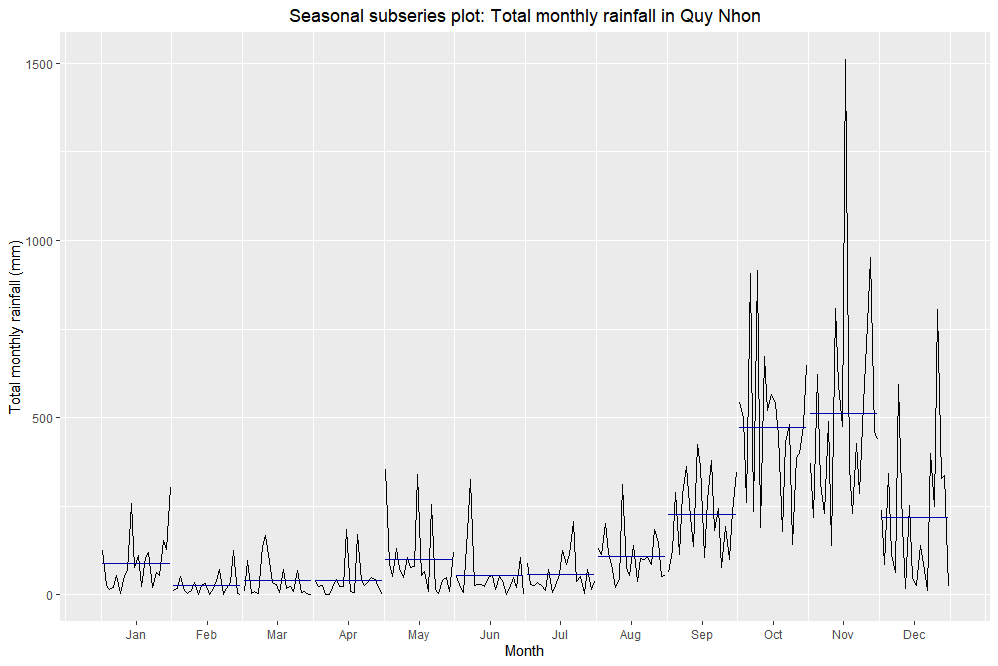
\includegraphics[width=1\linewidth,height=6cm]{V4} 
	\end{figure}
\end{frame}

\begin{frame}{2.3 Phân tích và dự báo lượng mưa tại trạm quan trắc Quy Nhơn.}
	\begin{figure}[!htb]
		\centering
		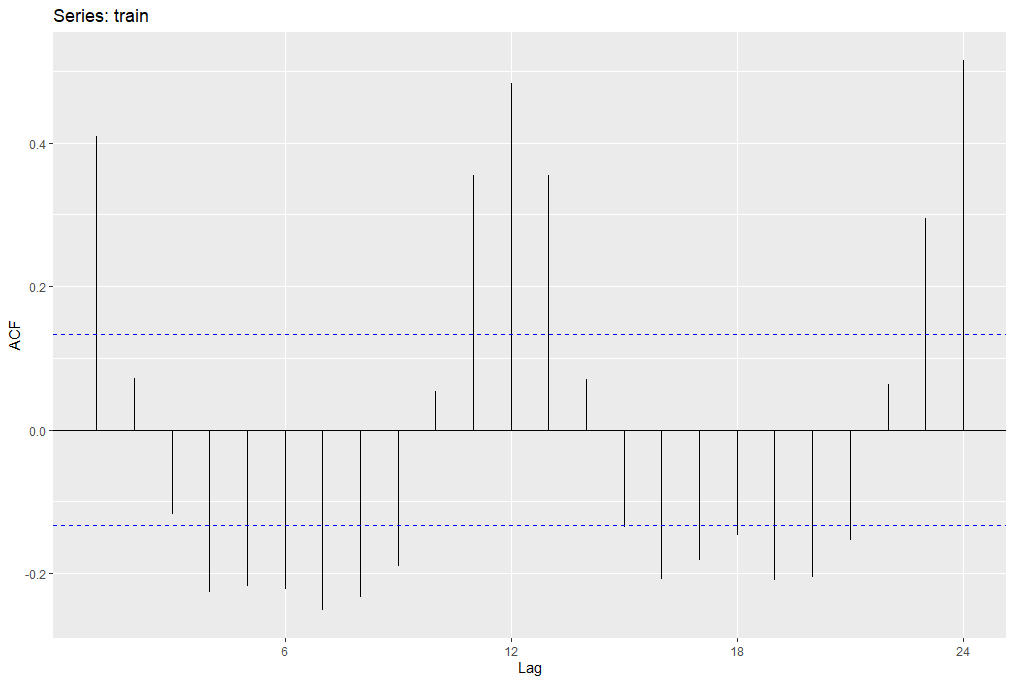
\includegraphics[width=1\linewidth,height=6cm]{acfrainfall} 
	\end{figure}
\end{frame}

\begin{frame}{2.3 Phân tích và dự báo lượng mưa tại trạm quan trắc Quy Nhơn.}
	\textbf{Bước 2: Chuyển chuỗi không có tính dừng thành chuỗi có tính dừng}
	\begin{figure}[!htb]
		\centering
		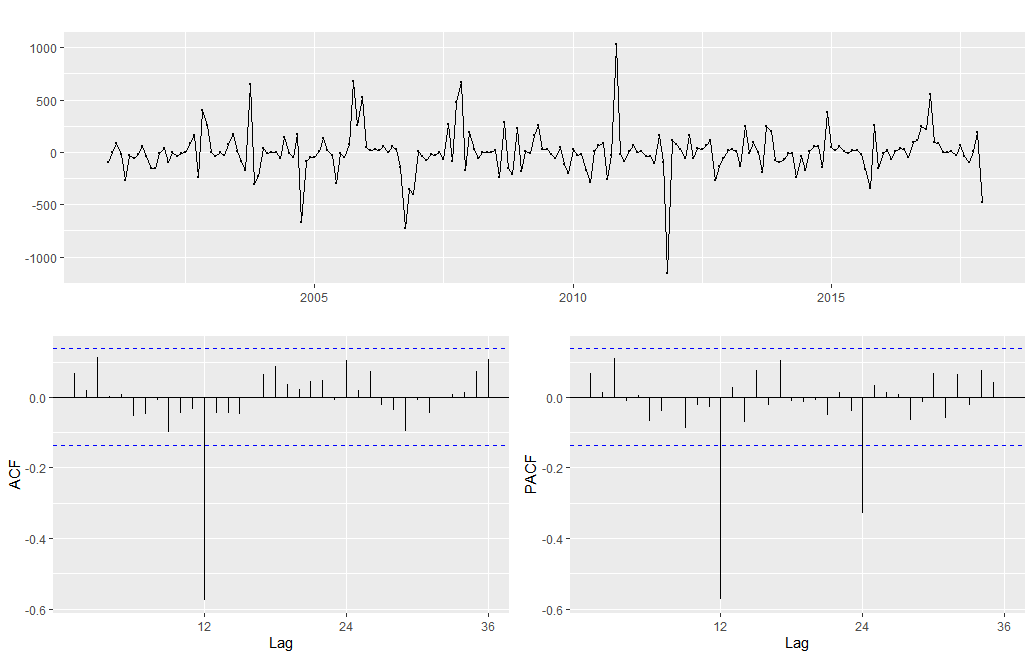
\includegraphics[width=1\linewidth,height=6cm]{V6} 
	\end{figure}
\end{frame}

\begin{frame}{2.3 Phân tích và dự báo lượng mưa tại trạm quan trắc Quy Nhơn.}
	\textbf{Bước 2: Chuyển chuỗi không có tính dừng thành chuỗi có tính dừng}
	\begin{figure}[!htb]
		\centering
		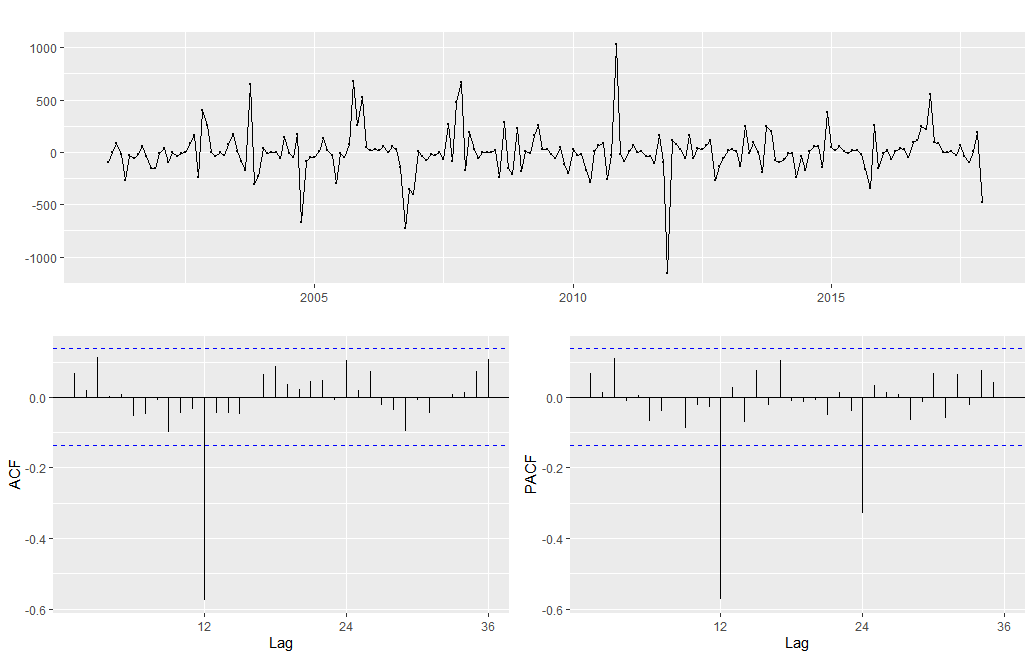
\includegraphics[width=1\linewidth,height=6cm]{V6} 
	\end{figure}
\end{frame}

\begin{frame}{2.3 Phân tích và dự báo lượng mưa tại trạm quan trắc Quy Nhơn.}
	\textbf{Bước 2: Chuyển chuỗi không có tính dừng thành chuỗi có tính dừng}
	\begin{figure}[!htb]
		\centering
		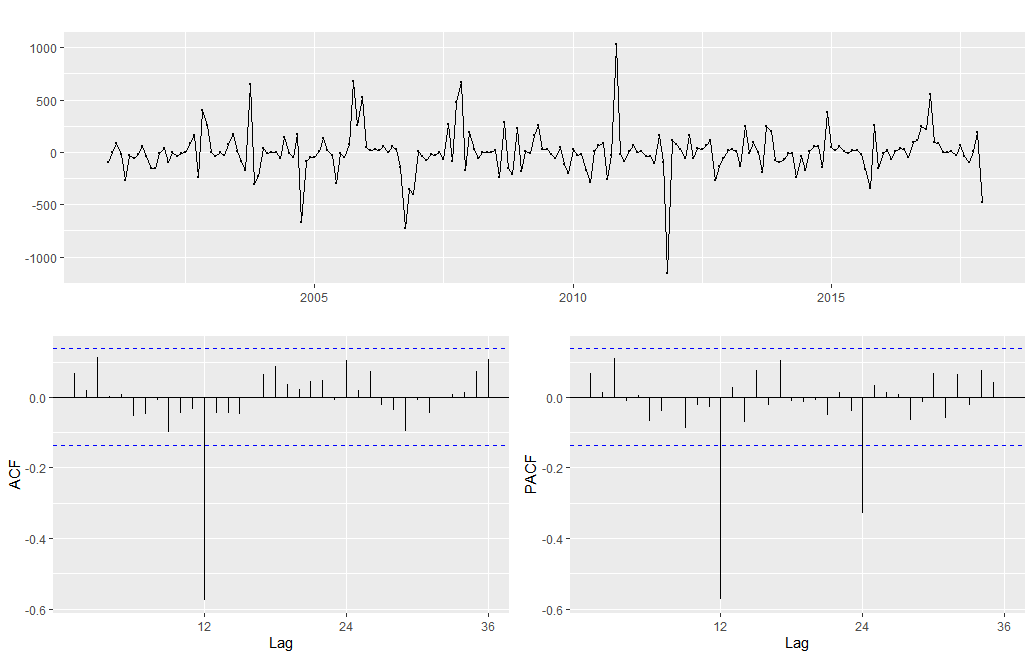
\includegraphics[width=1\linewidth,height=6cm]{V6} 
	\end{figure}
\end{frame}

\begin{frame}{2.3 Phân tích và dự báo lượng mưa tại trạm quan trắc Quy Nhơn.}
	\textbf{Bước 3: Chọn mô hình thích hợp từ đồ thị ACF và PACF}
	\begin{figure}[!htb]
		\centering
		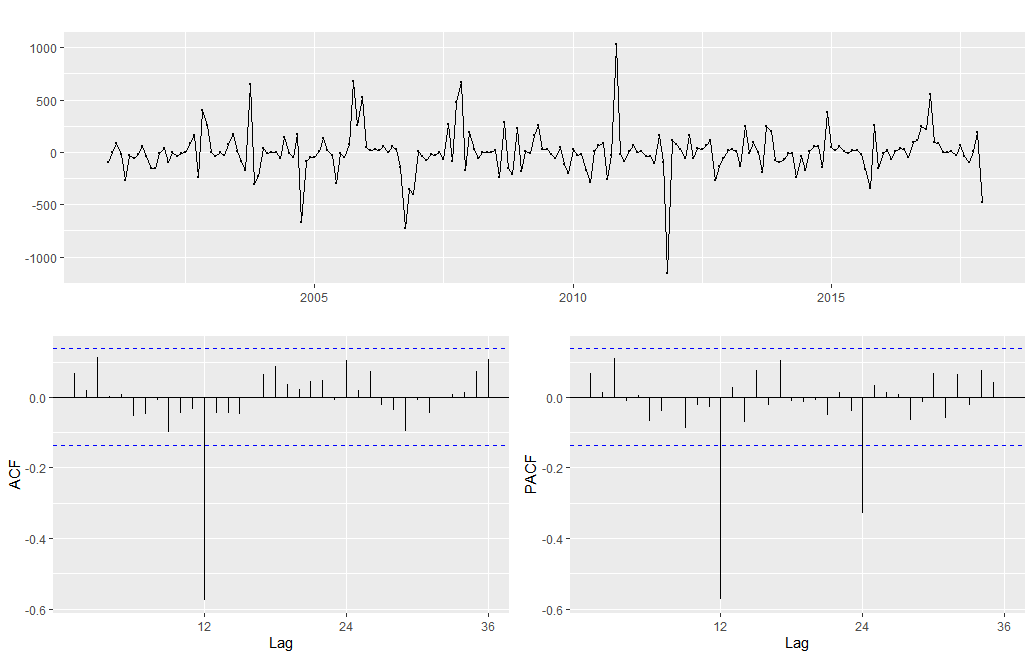
\includegraphics[width=1\linewidth,height=5cm]{V6} 
	\end{figure}
\textsc{\bf{ACF $\Longrightarrow$ ARIMA(0,0,0)(0,1,1)$_{12}$ [AICc=2648.02]}}\\
\pause
PACF $\Longrightarrow$ ARIMA(0,0,0)(0,1,2)$_{12}$ [AICc=2648.89]
\end{frame}

\begin{frame}{2.3 Phân tích và dự báo lượng mưa tại trạm quan trắc Quy Nhơn.}
	\textbf{Bước 4: Khớp  ARIMA(0,0,0)(0,1,1)$_{12}$ và chọn mô hình phù hợp nhất}\\
	\begin{figure}[!htb]
		\centering
		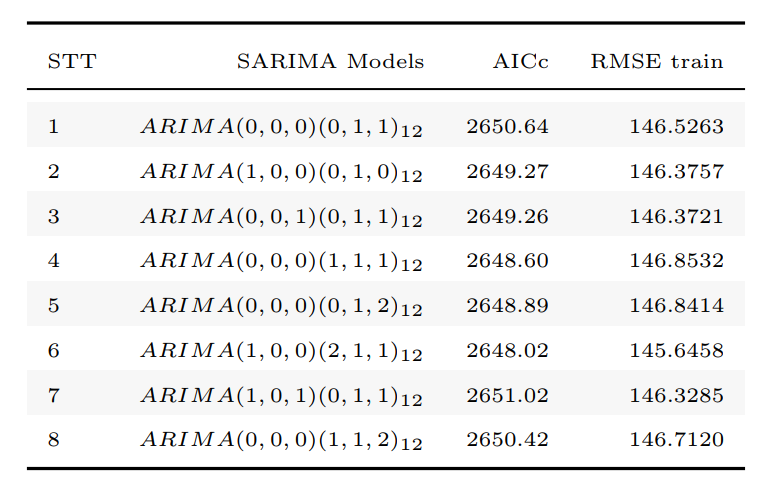
\includegraphics[width=1\linewidth,height=5.5cm]{duong8} 
	\end{figure}
\end{frame}

\begin{frame}{2.3 Phân tích và dự báo lượng mưa tại trạm quan trắc Quy Nhơn.}
	\textbf{Bước 5: Kiểm tra phần dư từ mô hình ARIMA(1,0,0)(2,1,1)$_{12}$}\\
	\begin{figure}[!htb]
		\centering
		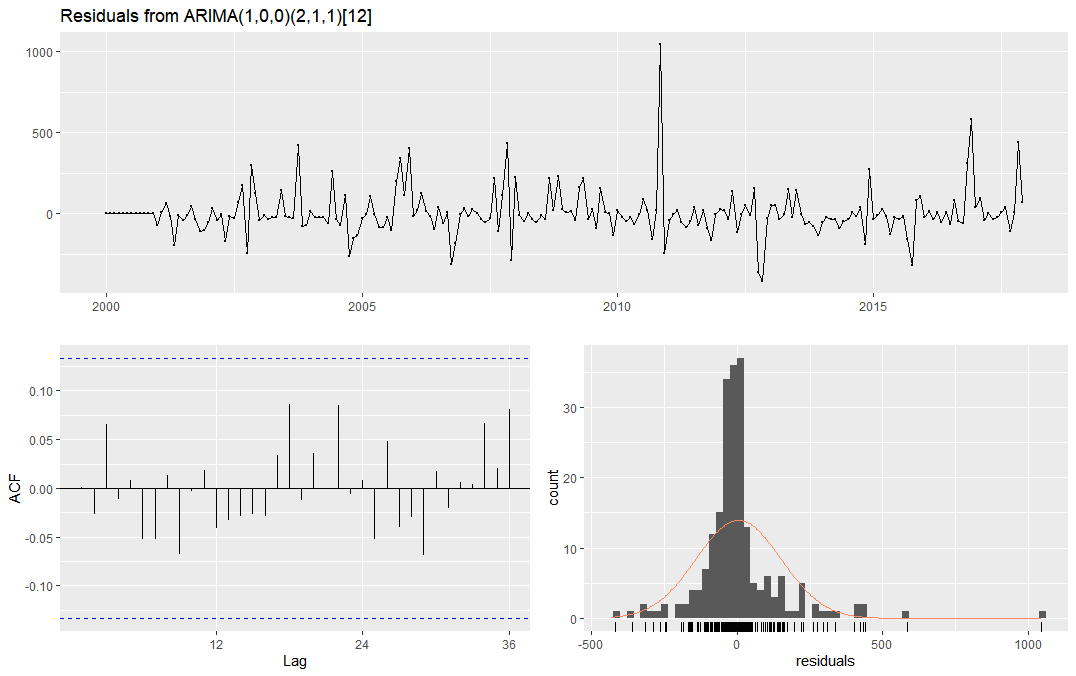
\includegraphics[width=1\linewidth,height=5.5cm]{V7} 
	\end{figure}
\end{frame}

\begin{frame}{2.3 Phân tích và dự báo lượng mưa tại trạm quan trắc Quy Nhơn.}
	\textbf{Bước 6: Đánh giá sai số từ mô hình ARIMA(1,0,0)(2,1,1)$_{12}$ và dự báo}\\
	\begin{figure}[!htb]
		\centering
		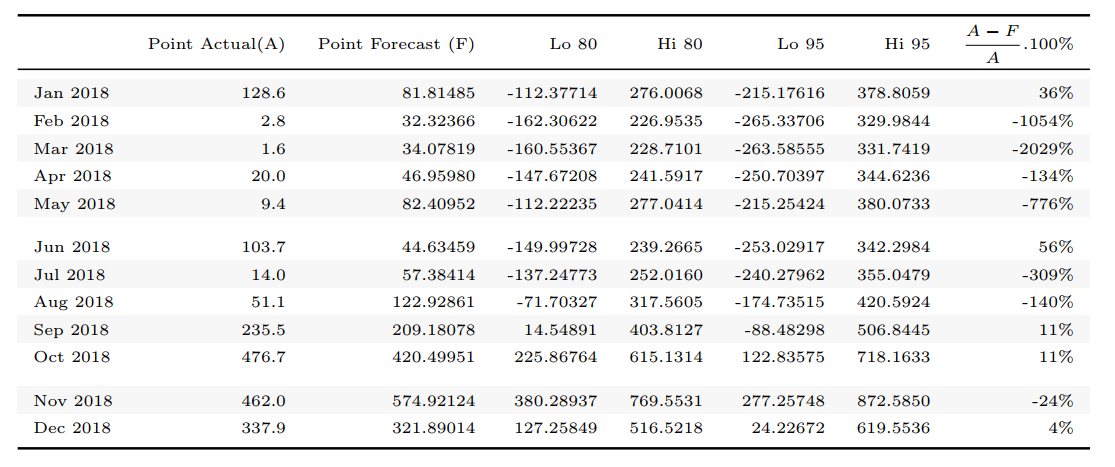
\includegraphics[width=1\linewidth,height=5.5cm]{duong9} 
	\end{figure}
\end{frame}

\begin{frame}{2.3 Phân tích và dự báo lượng mưa tại trạm quan trắc Quy Nhơn.}
	\begin{figure}[!htb]
		\centering
		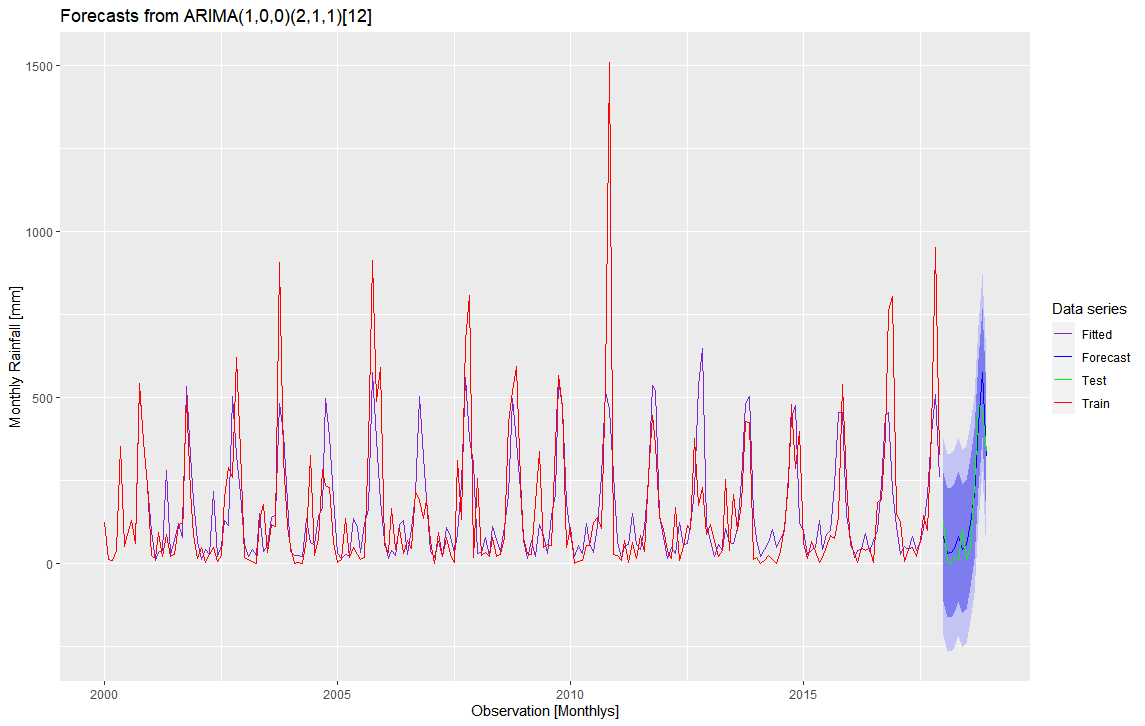
\includegraphics[width=1\linewidth,height=5.5cm]{V8} 
	\end{figure}
\end{frame}

\begin{frame}{2.3 Phân tích và dự báo lượng mưa tại trạm quan trắc Quy Nhơn.}
	\textbf{Sự chênh lệch lớn lượng mưa hàng tháng ở mùa khô là do đâu?}\\
	\pause
	\begin{itemize}
\item Một số quá trình xảy ra trong khoảng thời gian ngắn, như sự phát triển của hệ thống synop trong khí quyển là một trong những nguyên nhân dẫn đến sai số dự báo mùa.
	\pause 
\item ENSO là nhân tố ảnh hưởng lớn nhất đến các dao động khí hậu hàng năm, chính sự kết hợp này là nguồn gốc chính sinh ra dị thường về nhiệt độ và lượng mưa trên phạm vi toàn cầu.
	\end{itemize}
\end{frame}

\begin{frame}{2.3 Phân tích và dự báo lượng mưa tại trạm quan trắc Quy Nhơn.}
	\textbf{Bước 6: Đánh giá sai số từ mô hình ARIMA(1,0,0)(2,1,1)$_{12}$ và dự báo}\\
	\begin{figure}[!htb]
		\centering
		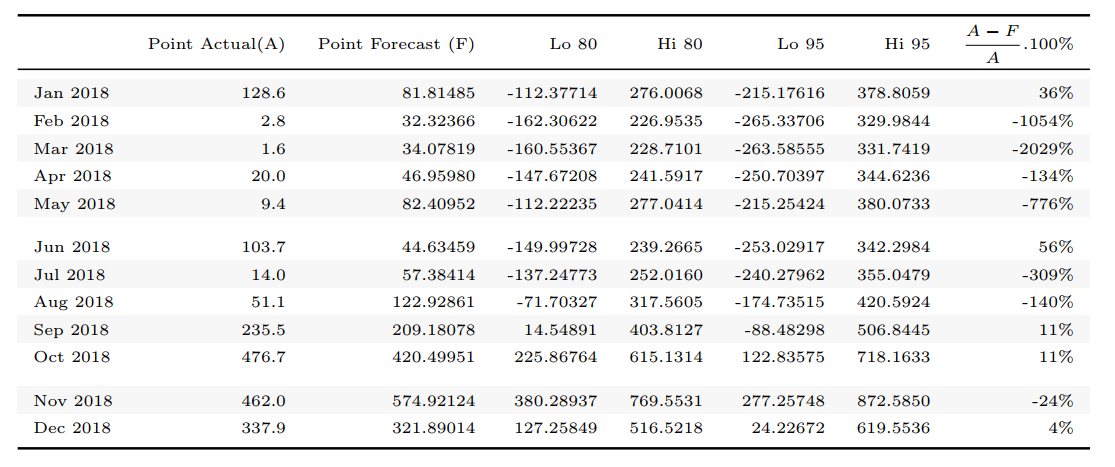
\includegraphics[width=1\linewidth,height=5.5cm]{duong9} 
	\end{figure}
\end{frame}

\begin{frame}{2.3 Phân tích và dự báo lượng mưa tại trạm quan trắc Quy Nhơn.}
	\begin{figure}[!htb]
		\centering
		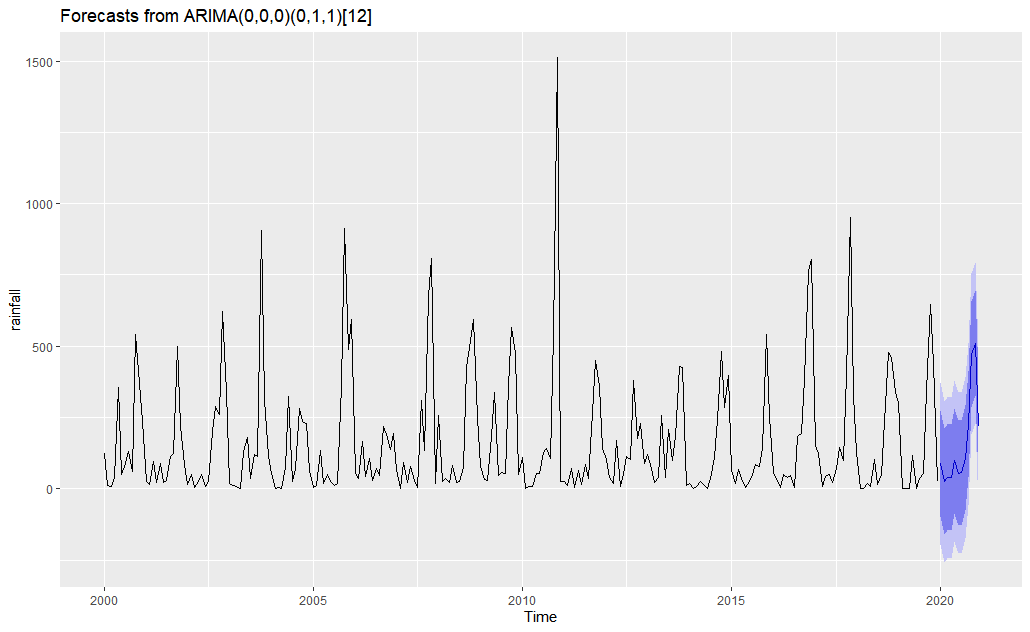
\includegraphics[width=1\linewidth,height=5cm]{V9} 
		\caption{Đồ thị dự báo lượng mưa theo tháng cho năm 2019 và 2020}
	\end{figure}
\end{frame}

\begin{frame}{2.4 Website Dashboard COVID-19}
\url{https://nguyenquocduong.shinyapps.io/NCKH/}	
\pause
	\begin{figure}[!htb]
		\centering
		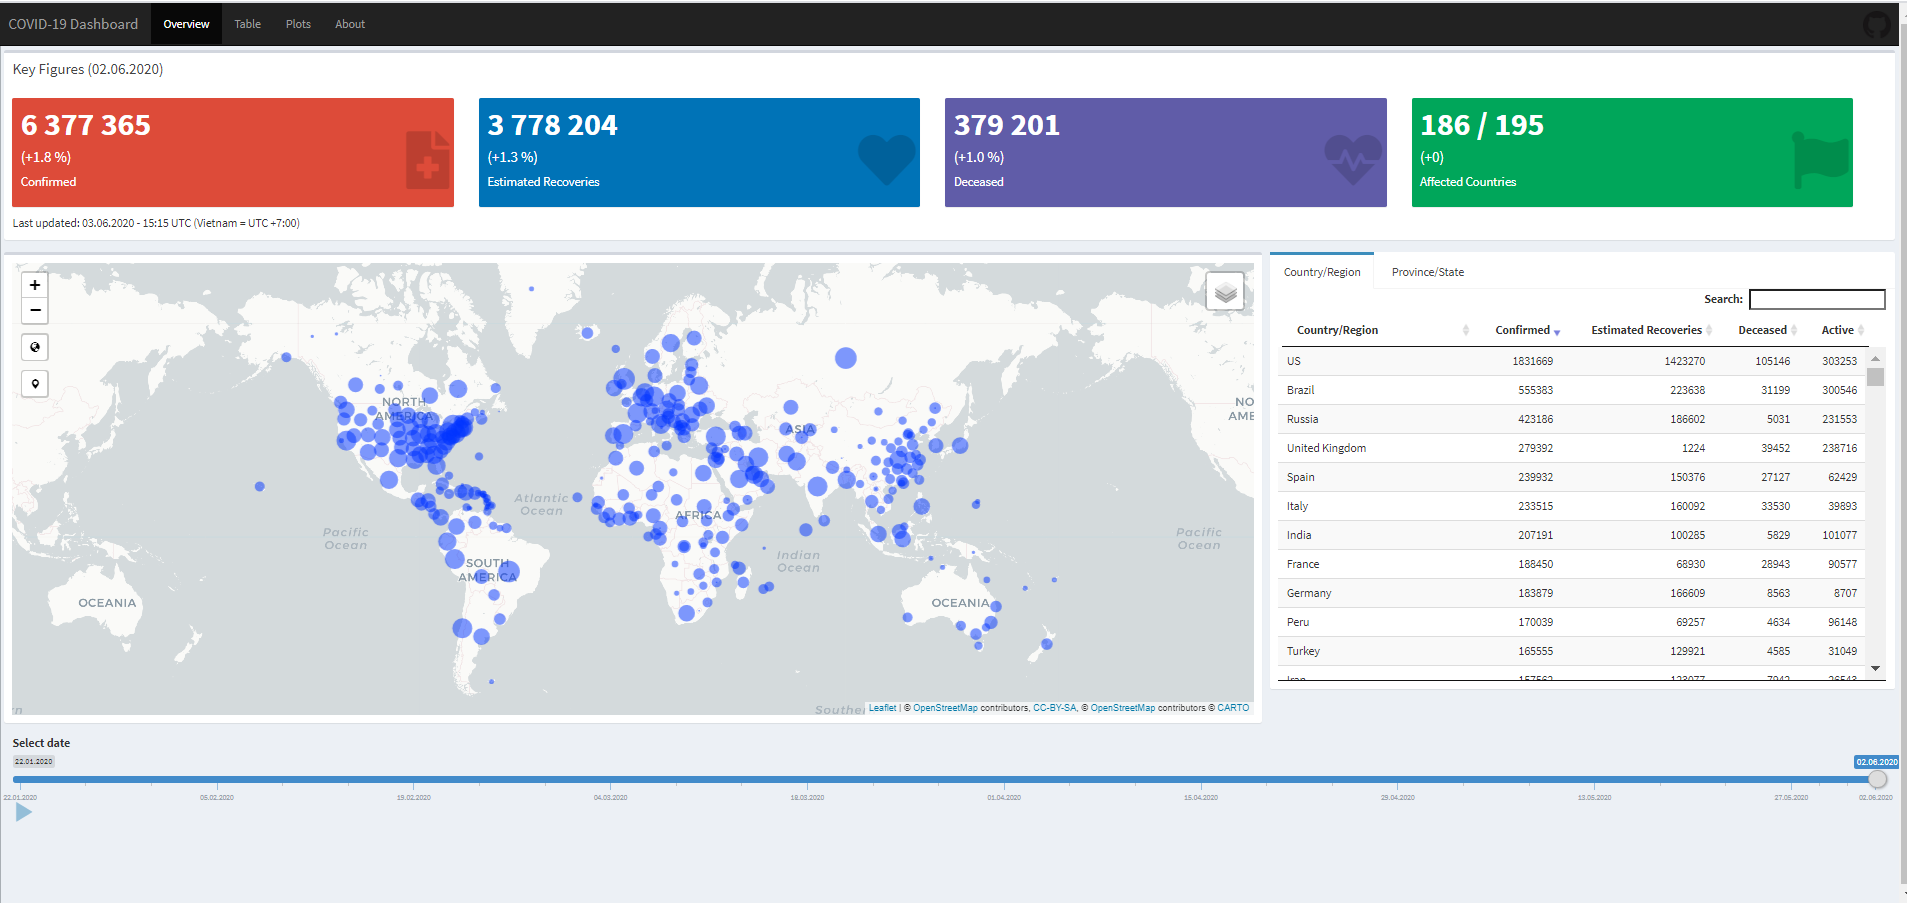
\includegraphics[width=1\linewidth,height=6cm]{duong10} 
	\end{figure}
\end{frame}

\begin{frame}{2.5 So sánh mô hình ARIMA và NNAR}
So sánh mô hình ARIMA và \textit{mô hình mạng noron tự hồi quy NNAR (Neural Retwork Auto-Regression)} trên tập dữ liệu lượng mưa hàng tháng tại trạm quan trắc Quy Nhơn dựa vào các thước đo sai số trên tập "test".
\end{frame}

\begin{frame}{2.5 So sánh mô hình ARIMA và NNAR}
	\begin{figure}[!htb]
	\centering
	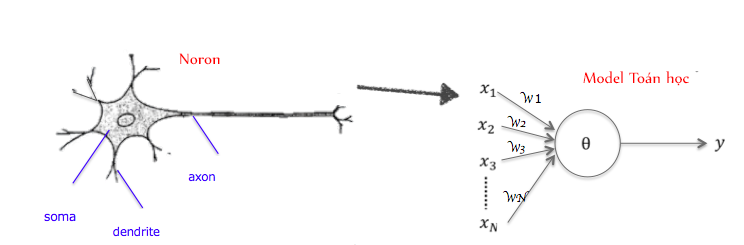
\includegraphics[width=1\linewidth,height=6cm]{noron} 
\end{figure}
\end{frame}

\begin{frame}{2.5 So sánh mô hình ARIMA và NNAR}
Hàm tổ hợp tuyến tính có dạng tổng quát
\begin{align*}
y_t = a_t + \sum_{i =1}^{n}w_{i, t}x_t.
\end{align*}
\end{frame}

\begin{frame}{2.5 So sánh mô hình ARIMA và NNAR}
Trong tầng ẩn (hidden layer), khi đó $y_t$ được điều chỉnh với việc sử dụng một hàm phi tuyến, chẳng hạn hàm sigmoid
\begin{align*}
f(y_t) = \frac{1}{1+e^{-y_t}},
\end{align*}
để nhận được giá trị đầu vào cho tầng kế tiếp.
\end{frame}

\begin{frame}{2.5 So sánh mô hình ARIMA và NNAR}
Đối với dữ liệu có tính mùa vụ, ta có mô hình NNAR($p$, $P$, $k$)$_m$ tổng quát với các đầu vào là $(y_{t-1}, y_{t-2},\dots, y_{t-p}, y_{t-m}, y_{t-2m}, y_{t-Pm})$ và $k$ noron tầng ẩn. Mô hình NNAR($p$, $P$, 0)$_m$ là tương đương với mô hình ARIMA($p$, 0, 0)($P$, 0, 0)$_m$ nhưng không có các giới hạn về các tham số để đảm bảo tính dừng.
\end{frame}

\begin{frame}{2.5 So sánh mô hình ARIMA và NNAR}
	\begin{figure}[!htb]
		\centering
		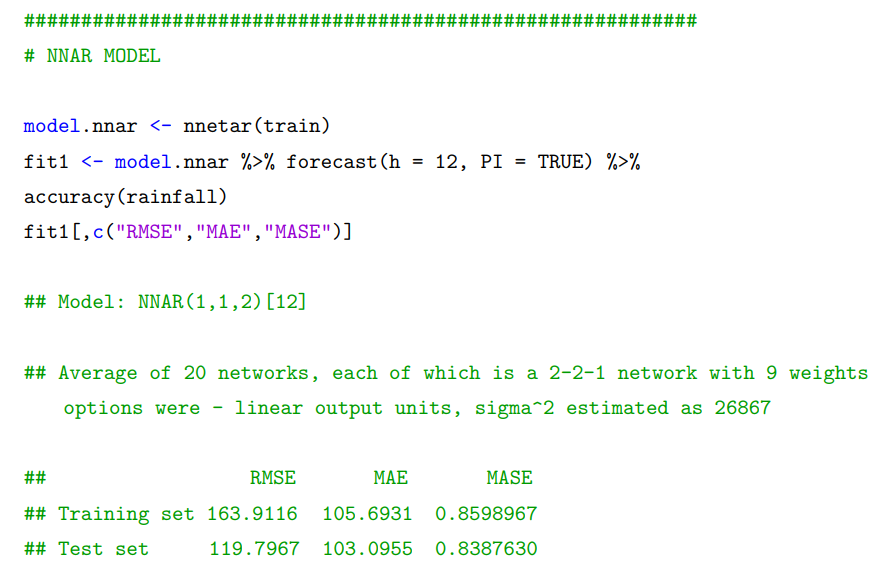
\includegraphics[width=1\linewidth,height=6cm]{duong11} 
	\end{figure}
\end{frame}

\begin{frame}{2.5 So sánh mô hình ARIMA và NNAR}
	\begin{figure}[!htb]
		\centering
		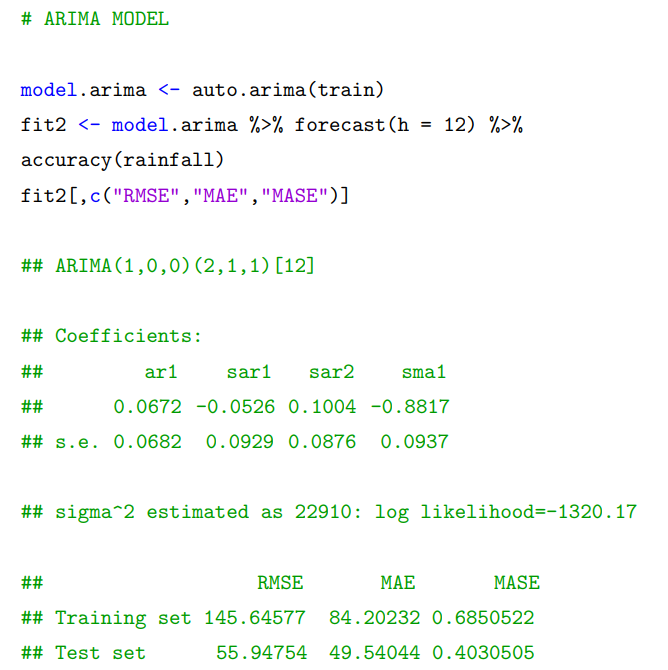
\includegraphics[width=1\linewidth,height=6cm]{duong12} 
	\end{figure}
\end{frame}

\begin{frame}{2.5 So sánh mô hình ARIMA và NNAR}
NNAR MODEL
	\begin{figure}[!htb]
	\centering
	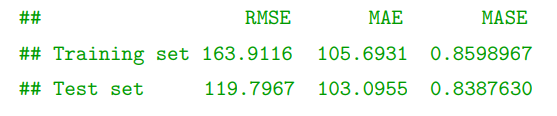
\includegraphics[width=1\linewidth,height=2.5cm]{duong13} 
\end{figure}
ARIMA MODEL
	\begin{figure}[!htb]
	\centering
	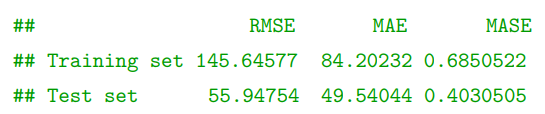
\includegraphics[width=1\linewidth,height=2.5cm]{duong14} 
\end{figure}
\end{frame}

\begin{frame}{THẢO LUẬN}
\textbf{Những mặt thuận lợi khi sử dụng mô hình ARIMA}
\begin{enumerate}
\item ARIMA là một trong những mô hình tuyến tính phổ biến nhất trong dự báo chuỗi thời gian đã được áp dụng rộng rãi trong thập kỷ qua.
\item ARIMA phát huy thế mạnh trong việc sử dụng để dự báo tài chính, chứng khoán, kinh tế lượng, khí tượng thủy văn, \dots
\item ARIMA thích hợp cho các bài toán dự báo ngắn hạn.
\item Hơn nữa, ARIMA còn là nền tảng để xây dựng các mô hình lai phù hợp với từng loại dữ liệu cụ thể và cho kết quả chính xác hơn như ARIMA-ANN, ARIMA-LSTM, ARIMAX, \dots
\end{enumerate}
\end{frame}

\begin{frame}{\center{THẢO LUẬN}}
\textbf{Những mặt hạn của mô hình ARIMA}
\begin{enumerate}
	\item Trong ARIMA, một cấu trúc tương quan tuyến tính được giả định giữa các giá trị trong chuỗi thời gian. Do đó, ARIMA chỉ phát hiện được các khuôn mẫu tuyến tính có trong chuỗi dữ liệu còn khuôn mẫu không tuyến tính thì không được phát hiện. 
\item Các giá trị trong tương lai được dự báo phụ thuộc vào quá khứ nên đối với bài toán dự báo dài hạn, việc lựa chọn ARIMA là không phù hợp.
\end{enumerate}
\end{frame}

\begin{frame}{KẾT LUẬN VÀ KIẾN NGHỊ} 
\textbf{Trong đề tài này, chúng tôi đã đạt được một số kết quả sau:} 
\begin{enumerate}
\item Tìm hiểu lý thuyết căn bản, quan trọng về chuỗi thời gian, hồi quy cổ điển với chuỗi thời gian và mô hình ARIMA.
\item Bước đầu đã nắm vững cách sử dụng các lệnh trong R để xây dựng mô hình ARIMA; hiểu và giải thích được kết quả đầu ra của mô hình ARIMA, cũng như nắm được kỹ năng về xử lý số liệu thô và kỹ năng vẽ hình, biểu đồ bằng phần mềm R.
\item Hơn nữa, chúng tôi đã xây dựng một website Dashboard COVID-19 nhằm theo dõi và kiểm soát tình hình dịch bệnh trên toàn cầu bằng phần mềm R.
\item Đồng thời, trong quá trình làm phần ví dụ thực hành với R, chúng tôi đã có điều kiện tìm hiểu thêm nhiều kiến thức mới ở các lĩnh vực khác nhau (ứng với từng ví dụ như: dịch tễ học, chăm sóc sức khỏe, khí tượng thủy văn, ...
\end{enumerate}
\end{frame}

\begin{frame}{Tài liệu tham khảo}
\begin{thebibliography}{99}
	\bibitem{1} R. H. Shumway and D. S. Stoffer, \textbf{\textit{Time Series Analysis and Its Applications}}, Springer Publisher, USA(2006).
	\bibitem{2} G. E. P. Box, G. M. Jenkins, G. C. Reinsel and G. M. Liung, \textbf{\textit{Time Series Analysis: Forecasting and Control, $5^{th}$ edition}}, Publisher Wiley, Canada(2016).
	\bibitem{3} R. J. Hyndman and G. Athanasopoulos, \textbf{\textit{Forecasting: Principles and Practice, $2^{nd}$ edition}}, OTexts Publisher, USA(2018).
	\bibitem{4} R. Krispin,  \textbf{\textit{Hands-On Time Series Analysis with R}}, Packt Publisher, UK(2019). 
\end{thebibliography}	
\end{frame}

\begin{frame}
\begin{thebibliography}{99}	
	\bibitem{5} G. James, D. Witten, T. Hastie and R. Tibshirani, \textbf{\textit{An Introduction to Statistical Learning with Applications in R, 1st edition}}, Springer Texts in Statistics, USA(2007)
	\bibitem{6} Nguyễn Văn Tuấn,  \textbf{\textit{Phân tích dữ liệu với R}}, NXB Tổng hợp T.P Hồ Chí Minh, 2014.
	\bibitem{7} Nguyễn Chí Dũng, \textbf{\textit{Kinh tế lượng ứng dụng với R}}, Ebook, 2017.
	\bibitem{8} R. J. Hyndman, \textbf{\textit{Forecasting Functions for Time Series and Linear Models}}, CRAN, 2020.
	\bibitem{9} Nguyễn Duy Tiến và Vũ ngọc Yên, \textbf{\textit{Lý thuyết xác suất}}, NXB Giáo dục, 2000.
\end{thebibliography}	
\end{frame}

\begin{frame}
\begin{thebibliography}{99}	
	\bibitem{10} Luz PM, Mendes BV, Codeco CT, Struchiner CJ and Galvani AP, \textbf{\textit{Time series analysis of dengue incidence in Rio de Janeiro}}, , Am J Trop Med Hyg, Brazil(2008), 79 (6): 933-939.
	\bibitem{11} Earnest A, Chen MI, Ng D and Leo YS, \textbf{\textit{Using autoregressive integrated moving average(ARIMA) models to predict and monitor the number of beds occupied during a SARS outbreak in a tertiary hospital in Singapore}}, BMC Health Services Research, (2005), 5: 36-10.
	\bibitem{12}  Li XJ, Kang DM, Cao J and Wang JZ, \textbf{\textit{A time series model in incidence forecasting of hemorrhagic fever with renal syndrome}}, Journal of Shandong University (Health Sciences), (2008), 46 (5): 547-549.
\end{thebibliography}	
\end{frame}

\begin{frame}
\begin{thebibliography}{99}
	\bibitem{13}  K. Mizumoto , K. Kagaya , A. Zarebski and G. Chowell, \textbf{\textit{Estimating the asymptomatic proportion of coronavirus disease 2019 (COVID-19) cases on board the Diamond Princess cruise ship, Yokohama, Japan, 2020}},  Euro Surveill, 2020, 25(10).
    \bibitem{14} C. Wang, L. Liu, X. Hao, H. Guo, Q. Wang, J. Huang, N. He, H. Yu, X. Lin, A. Pan, S. Wei and T. Wu, \textbf{\textit{Evolving Epidemiology and Impact of Non-pharmaceutical Interventions on the Outbreak of Coronavirus Disease 2019 in Wuhan, China}}, The Preprint Server for Healthy Sciences, 2020.
    \bibitem{15} R. Li, S. Pei, B. Chen, Y. Song, T. Zhang, W. Yang and J Shaman, \textbf{\textit{Substantial undocumented infection facilitates the rapid dissemination of novel coronavirus (SARS-CoV2)}}, Science, 2020.
\end{thebibliography}	
\end{frame}

\begin{frame}
	\begin{thebibliography}{99}
	\bibitem{16} S. Boccia, W. Ricciardi and J. P. A. Ioannidis, \textbf{\textit{What Other Countries Can Learn From Italy During the COVID-19 Pandemic}}, JAMA Intern Med. Published online April 07, 2020. 
	\bibitem{17} E.M. Rasmusson and T.H. Carpenter, \textbf{\textit{The relationship between eastern equatorial Pacific SSTs and rainfall over India and Sri Lanka}}, Mon. Wea. Rev, 1983, 517-528.
	\bibitem{18} C.F. Ropelewski and M.S. Halpert, “\textbf{\textit{Global and Regional Scale Precipitation Patterns Associated with the El Niño/Southern Oscillation}}, Mon Wea Rev, 1987, 1606-1626.
	\bibitem{19} Website:\newblock{\textcolor{blue}{\url{http://www.nguyenquocduong.github.com}}}.
\end{thebibliography}	
\end{frame}

\begin{frame}
\centerline{\Large\bf \fontsize{18}{18}\selectfont{\color{red}{KẾT THÚC BÁO CÁO}}}
\vspace{1cm}
\centerline{\Large\bf \fontsize{23}{18}\selectfont{\color{blue}{TRÂN TRỌNG CẢM ƠN!}}}
\end{frame}
\end{document} 
